% Capitolul 7: Cointegrare și VECM
% Serii de timp -- Programele de licență Informatică economică și Cibernetică economică, Academia de Studii Economice din București
% GENERAT de latex/build_chapter7.py -- modificați generatorul, nu acest fișier.

\newcommand{\coursename}{Serii de timp}
\def\tsalang{ro}
% Preambul comun TSA -- Serii de timp / Time Series Analysis (Beamer, 16:9)
% Același design ca MFM și SFM (preluat din SFM, 5 octombrie 2026). Înainte de % Preambul comun TSA -- Serii de timp / Time Series Analysis (Beamer, 16:9)
% Același design ca MFM și SFM (preluat din SFM, 5 octombrie 2026). Înainte de % Preambul comun TSA -- Serii de timp / Time Series Analysis (Beamer, 16:9)
% Același design ca MFM și SFM (preluat din SFM, 5 octombrie 2026). Înainte de \input{../../latex/preamble} se definește
%   \newcommand{\coursename}{Time Series Analysis}      (EN)
%   \newcommand{\coursename}{Serii de timp}       (RO)  și  \def\tsalang{ro}
% Fișierele .tex se află în EN/Courses, EN/Seminars, RO/Cursuri, RO/Seminarii (două niveluri sub rădăcină).
% Deck-urile sînt generate de latex/build_chapterN.py / build_seminarN.py (vezi latex/tsa_build.py).

\documentclass[9pt, aspectratio=169, t]{beamer}
\providecommand{\coursename}{Time Series Analysis}

% Ensure content fits on slides
\setbeamersize{text margin left=8mm, text margin right=8mm}
% Smaller institute font (title page)
\setbeamerfont{institute}{size=\footnotesize}

%=============================================================================
% THEME AND STYLE CONFIGURATION
%=============================================================================
\usetheme{default}
% Using default theme for clean header/footer control

% Color Palette (matching Redispatch PDF)
\definecolor{MainBlue}{RGB}{26, 58, 110}
\definecolor{AccentBlue}{RGB}{26, 58, 110}
\definecolor{IDAred}{RGB}{205, 0, 0}
\definecolor{DarkGray}{RGB}{51, 51, 51}
\definecolor{MediumGray}{RGB}{128, 128, 128}
\definecolor{LightGray}{RGB}{248, 248, 248}
\definecolor{VeryLightGray}{RGB}{235, 235, 235}
\definecolor{KeynoteGray}{RGB}{218, 218, 218}
\definecolor{SectionGray}{RGB}{120, 120, 120}
\definecolor{FooterGray}{RGB}{100, 100, 100}
\definecolor{Crimson}{RGB}{220, 53, 69}
\definecolor{Forest}{RGB}{46, 125, 50}
\definecolor{Amber}{RGB}{181, 133, 63}
\definecolor{Orange}{RGB}{230, 126, 34}
\definecolor{Purple}{RGB}{142, 68, 173}

% Gradient background (exact Keynote 315° gradient: white to RGB 218,218,218)
\setbeamertemplate{background}{%
    \begin{tikzpicture}[remember picture, overlay]
        \shade[shading=axis, shading angle=315,
        top color=white, bottom color=KeynoteGray]
        (current page.south west) rectangle (current page.north east);
    \end{tikzpicture}%
}
% Fallback solid color for compatibility
\setbeamercolor{background canvas}{bg=}

\setbeamercolor{palette primary}{bg=MainBlue, fg=white}
\setbeamercolor{palette secondary}{bg=MainBlue!85, fg=white}
\setbeamercolor{palette tertiary}{bg=MainBlue!70, fg=white}
\setbeamercolor{structure}{fg=MainBlue}
\setbeamercolor{title}{fg=IDAred}
\setbeamercolor{frametitle}{fg=IDAred, bg=}
\setbeamercolor{block title}{bg=MainBlue, fg=white}
\setbeamercolor{block body}{bg=VeryLightGray, fg=DarkGray}
\setbeamercolor{block title alerted}{bg=Crimson, fg=white}
\setbeamercolor{block body alerted}{bg=Crimson!8, fg=DarkGray}
\setbeamercolor{block title example}{bg=Forest, fg=white}
\setbeamercolor{block body example}{bg=Forest!8, fg=DarkGray}
\setbeamercolor{item}{fg=MainBlue}

% Footer colors (override Madrid theme blue)
\setbeamercolor{author in head/foot}{fg=FooterGray, bg=}
\setbeamercolor{title in head/foot}{fg=FooterGray, bg=}
\setbeamercolor{date in head/foot}{fg=FooterGray, bg=}
\setbeamercolor{section in head/foot}{fg=FooterGray, bg=}
\setbeamercolor{subsection in head/foot}{fg=FooterGray, bg=}

% Bullet styles (apply everywhere including blocks)
\setbeamertemplate{itemize item}{\color{MainBlue}$\boxdot$}
\setbeamertemplate{itemize subitem}{\color{MainBlue}$\blacktriangleright$}
\setbeamertemplate{itemize subsubitem}{\color{MainBlue}\tiny$\bullet$}
\setbeamertemplate{itemize/enumerate body begin}{\normalsize}
\setbeamertemplate{itemize/enumerate subbody begin}{\normalsize}

% Item spacing - compact style
\setlength{\leftmargini}{10pt}       % Level 1: minimal indent
\setlength{\leftmarginii}{10pt}      % Level 2: minimal additional indent
% Compact list spacing (zero extra space before/after lists in blocks)
\makeatletter
\def\@listi{\leftmargin\leftmargini \topsep 0pt \parsep 0pt \itemsep 0pt}
\def\@listii{\leftmargin\leftmarginii \topsep 0pt \parsep 0pt \itemsep 0pt}
\makeatother

\setbeamertemplate{navigation symbols}{}

%=============================================================================
% CUSTOM HEADLINE
%=============================================================================
\setbeamertemplate{headline}{%
    \vskip10pt%
    \hbox to \paperwidth{%
        \hskip0.5cm%
        {\small\color{FooterGray}\renewcommand{\hyperlink}[2]{##2}\insertsectionhead}%
        \hfill%
        \textcolor{FooterGray}{\small\insertframenumber}%
        \hskip0.5cm%
    }%
    \vskip4pt%
    {\color{FooterGray}\hrule height 0.4pt}%
}

%=============================================================================
% CUSTOM FOOTER
%=============================================================================
\usepackage{fontawesome5}

\setbeamertemplate{footline}{%
    {\color{FooterGray}\hrule height 0.4pt}%
    \vskip4pt%
    \hbox to \paperwidth{%
        \hskip0.5cm%
        \textcolor{FooterGray}{\small\coursename}%
        \hfill%
        \raisebox{-0.1em}{%
            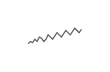
\begin{tikzpicture}[x=0.08em, y=0.08em, line width=0.4pt]
                \draw[FooterGray] (0,3) -- (1,4) -- (2,3.5) -- (3,5) -- (4,4) -- (5,6) -- (6,5.5) -- (7,4) -- (8,5) -- (9,7) -- (10,6) -- (11,5) -- (12,6.5) -- (13,8) -- (14,7) -- (15,6) -- (16,7.5) -- (17,9) -- (18,8) -- (19,7) -- (20,8.5) -- (21,10) -- (22,9) -- (23,8) -- (24,9.5);
            \end{tikzpicture}%
        }%
        \hskip0.5cm%
    }%
    \vskip6pt%
}

%=============================================================================
% PACKAGES
%=============================================================================
\usepackage[utf8]{inputenc}
\DeclareUnicodeCharacter{03B1}{\ensuremath{\alpha}}
\usepackage[T1]{fontenc}
\usepackage{amsmath, amssymb, amsthm}
\usepackage{mathtools}
\usepackage{bm}
\usepackage{tikz}
\usetikzlibrary{arrows.meta, positioning, shapes, calc, decorations.pathreplacing, shadings}
\usepackage{booktabs}
\usepackage{multirow}
\usepackage{array}
\usepackage{graphicx}
\usepackage{animate}
\usepackage{hyperref}
\usepackage{colortbl}
\usepackage{listings}
\lstset{language=Python, basicstyle=\ttfamily\scriptsize, keywordstyle=\color{MainBlue}\bfseries,
  commentstyle=\color{Forest}, stringstyle=\color{Crimson}, breaklines=true,
  frame=none, backgroundcolor=\color{VeryLightGray}, xleftmargin=2mm}
\hypersetup{colorlinks=true, linkcolor=MainBlue, urlcolor=MainBlue}
\graphicspath{{../../logos/}{../../charts/}{../../photos/}}
\usepackage{xcolor}
\hfuzz=2pt  % Suppress tiny overfull warnings (<2pt)
\vfuzz=2pt  % Suppress tiny vertical overfull warnings (<2pt)
% \mathrm in the sans-serif family of the slides (beamer resets \mathrm to the serif family at \begin{document};
% this hook runs after beamer's, so WN, Var, RMSE, ... in formulas match the surrounding text)
% Bold vectors and matrices in the same sans-serif family: \mathbf{A} in sans bold (beamer's own \mathbf came out in
% medium weight), and the bold upright Greek capitals of \boldsymbol / \bm (\bSigma, \bPhi, \boldsymbol{\Theta}) in
% cmss bold: bm.sty fixes its "boldoperators" font when it is loaded (serif cmbx), before beamer switches the
% operators to cmss, so it is reset here.
\AtBeginDocument{%
  \SetMathAlphabet{\mathrm}{normal}{\encodingdefault}{\sfdefault}{\mddefault}{n}%
  \SetMathAlphabet{\mathrm}{bold}{\encodingdefault}{\sfdefault}{bx}{n}%
  \SetMathAlphabet{\mathbf}{normal}{\encodingdefault}{\sfdefault}{bx}{n}%
  \SetMathAlphabet{\mathbf}{bold}{\encodingdefault}{\sfdefault}{bx}{n}%
  \SetSymbolFont{boldoperators}{normal}{OT1}{cmss}{bx}{n}%
  \SetSymbolFont{boldoperators}{bold}{OT1}{cmss}{bx}{n}}

%=============================================================================
% QUANTLET COMMANDS
%   \quantlet{<displayed name>}{<url>}       (generic, compatible with the older TSA decks)
%   \tsaquantlet{Ch_05}{TSA_ch5_garch}       -> https://github.com/danpele/Time-Series-Analysis/tree/main/Quantlets/Ch_05/TSA_ch5_garch
%   \qlurl{<folder>} is defined per chapter by the generator (Quantlets/Ch_NN/<folder>)
%=============================================================================
\newcommand{\tsarepo}{https://github.com/danpele/Time-Series-Analysis}
\newcommand{\tsaqlbase}{https://github.com/danpele/Time-Series-Analysis/tree/main/Quantlets}
\newcommand{\quantlet}[2]{%
    \hfill\href{#2}{%
        \raisebox{-0.15em}{
\includegraphics[height=0.7em]{ql_logo.png}}%
        \textcolor{MainBlue}{\tiny\ #1}%
    }%
}
\newcommand{\tsaquantlet}[2]{\quantlet{\detokenize{#2}}{\tsaqlbase/#1/#2}}

%=============================================================================
% NOTEBOOKS (Google Colab)
%   \colaburl{notebooks/EN/chapter5_seminar_notebook.ipynb} -> the Colab link of a file in the TSA repo
%   \nb: the chapter notebook (each seminar deck redefines it with \renewcommand)
%=============================================================================
\newcommand{\colaburl}[1]{https://colab.research.google.com/github/danpele/Time-Series-Analysis/blob/main/#1}
\newcommand{\nb}{https://colab.research.google.com/github/danpele/Time-Series-Analysis/tree/main/notebooks/EN}
\newcommand{\nbname}{notebooks/EN}

%=============================================================================
% SLIDE HELPERS (used by the generators; the same as in MFM)
%=============================================================================
% local font size for list bodies (the preamble forces \normalsize)
\newcommand{\itemsize}[1]{\setbeamertemplate{itemize/enumerate body begin}{#1}\setbeamertemplate{itemize/enumerate subbody begin}{#1}}
\newcommand{\intitle}[1]{{\hypersetup{urlcolor=white}#1}}   % white links inside coloured title bars
\newcommand{\imgcap}[1]{{\scriptsize #1}\\[0.5mm]}          % caption under a photo
\newcommand{\imgcredit}[2]{{\tiny\color{FooterGray}\href{#1}{#2}}}   % image credit: source URL, author/licence
\newcommand{\aiprompt}[1]{{\ttfamily\color{MainBlue}#1}}     % a prompt to an AI assistant

%=============================================================================
% SEMINARS: student version by default; the instructor wrapper *_solutions.tex sets \solutionstrue
%=============================================================================
\makeatletter\@ifundefined{ifsolutions}{\expandafter\newif\csname ifsolutions\endcsname}{}\makeatother
\newcommand{\solonly}[1]{\ifsolutions #1\fi}
\newcommand{\propsub}{\ifsolutions\else\framesubtitle{\ifdefined\tsalang Rezolvarea se discută la seminar\else Solution discussed in class\fi}\fi}

%=============================================================================
% APPENDIX AND CHAPTER LINKS (latex/appendix_links.py writes the calls; it also re-declares these
% macros before \begin{document}, so the decks compile with or without this preamble block)
%=============================================================================
\providecommand{\tsaapplink}[3]{\hypertarget{#2}{}\hyperlink{#1}{\beamergotobutton{#3}}}
\providecommand{\tsaappback}[2]{\begin{tikzpicture}[remember picture,overlay]\node[anchor=south east] at ([xshift=-3mm,yshift=7mm]current page.south east){\hyperlink{#1}{\beamerreturnbutton{#2}}};\end{tikzpicture}}
\providecommand{\tsachlink}[2]{\href{#1}{#2}}
\providecommand{\tsachlinkt}[2]{\href{#1}{\usebeamercolor[fg]{frametitle}#2}}

%=============================================================================
% QUANTINAR COMMAND: link către un curs Quantinar (subiecte avansate)
%=============================================================================
\newcommand{\quantinar}[2]{%
    \href{#2}{%
        \raisebox{-0.15em}{
\includegraphics[height=0.8em]{qr_logo.png}}%
        \textcolor{MainBlue}{\scriptsize\ #1}%
    }%
}

%=============================================================================
% CUSTOM TITLE PAGE
%=============================================================================
\defbeamertemplate*{title page}{hybrid}[1][]
{
    \vspace{0.2cm}
    % Logos row - top header (with clickable links)
    \begin{center}
        \href{https://www.ase.ro}{
\includegraphics[height=1.0cm]{ase_logo.png}}\hspace{0.3cm}%
        \href{https://theida.net}{
\includegraphics[height=1.0cm]{ida_logo.png}}\hspace{0.3cm}%
        \href{https://blockchain-research-center.com}{
\includegraphics[height=1.0cm]{brc_logo.png}}\hspace{0.3cm}%
        \href{https://www.ai4efin.ase.ro}{
\includegraphics[height=1.0cm]{ai4efin_logo.png}}\hspace{0.3cm}%
        \href{https://ipe.ro/new}{
\includegraphics[height=1.0cm]{acad_logo.png}}\hspace{0.3cm}%
        \href{https://www.digital-finance-msca.com}{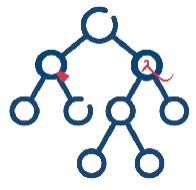
\includegraphics[height=1.0cm]{msca_logo.png}}%
    \end{center}

    \vspace{0.6cm}

    % Main title with Q logos on sides (with clickable links)
    \begin{center}
        \begin{minipage}{0.1\textwidth}
            \centering
            \href{https://quantlet.com}{
\includegraphics[height=1.1cm]{ql_logo.png}}
        \end{minipage}%
        \begin{minipage}{0.78\textwidth}
            \centering
            {\LARGE\bfseries\usebeamercolor[fg]{title}\inserttitle}

            \vspace{0.3cm}

            {\usebeamerfont{subtitle}\usebeamercolor[fg]{title}\insertsubtitle}
        \end{minipage}%
        \begin{minipage}{0.1\textwidth}
            \centering
            \href{https://quantinar.com}{
\includegraphics[height=1.1cm]{qr_logo.png}}
        \end{minipage}
    \end{center}

    \vspace{0.6cm}

    % Authors (left aligned)
    \hspace{0.5cm}{\usebeamerfont{author}\insertauthor}

    \vspace{0.3cm}

    % Institute/Affiliations (left aligned)
    \hspace{0.5cm}\begin{minipage}[t]{0.9\textwidth}
        \raggedright\small\insertinstitute
    \end{minipage}
}

%=============================================================================
% THEOREM ENVIRONMENTS
%=============================================================================
\theoremstyle{definition}
\setbeamertemplate{theorems}[numbered]
\ifdefined\tsalang
\newtheorem{defn}{Definiție}
\newtheorem{thm}{Teoremă}
\newtheorem{prop}{Propoziție}
\newtheorem{rmk}{Observație}
\else
\newtheorem{defn}{Definition}
\newtheorem{thm}{Theorem}
\newtheorem{prop}{Proposition}
\newtheorem{rmk}{Remark}
\fi

%=============================================================================
% CENTRED MINIPAGE (no extra vertical space)
%=============================================================================
\newenvironment{cminipage}[1]{%
    \par\noindent\hfill\begin{minipage}{#1}\ignorespaces
}{%
    \end{minipage}\hfill\null\par
}

%=============================================================================
% CUSTOM COMMANDS
%=============================================================================
\newcommand{\E}{\mathbb{E}}
\newcommand{\Var}{\text{Var}}
\newcommand{\Cov}{\text{Cov}}
\newcommand{\Corr}{\text{Corr}}
\newcommand{\R}{\mathbb{R}}
\newcommand{\N}{\mathbb{N}}
\newcommand{\Z}{\mathbb{Z}}
\newcommand{\B}{\mathbf{B}}
\newcommand{\imark}{\textcolor{MainBlue}{\textbullet}}
\newcommand{\RMSE}{\text{RMSE}}
\newcommand{\MAE}{\text{MAE}}
\newcommand{\MAPE}{\text{MAPE}}

% Boldface vector/matrix commands (VAR, VECM, state space; also used by the older TSA decks)
\newcommand{\bY}{\mathbf{Y}}
\newcommand{\bX}{\mathbf{X}}
\newcommand{\bA}{\mathbf{A}}
\newcommand{\bB}{\mathbf{B}}
\newcommand{\bepsilon}{\boldsymbol{\varepsilon}}
\newcommand{\bSigma}{\boldsymbol{\Sigma}}
\newcommand{\bPhi}{\boldsymbol{\Phi}}
\newcommand{\bGamma}{\boldsymbol{\Gamma}}
\newcommand{\bPi}{\boldsymbol{\Pi}}
\newcommand{\bc}{\mathbf{c}}
\newcommand{\balpha}{\boldsymbol{\alpha}}
\newcommand{\bbeta}{\boldsymbol{\beta}}
\newcommand{\bvarepsilon}{\boldsymbol{\varepsilon}}

% Legacy seminar marks (older TSA seminar decks)
\newcommand{\correct}{\textcolor{Forest}{\checkmark}}
\newcommand{\incorrect}{\textcolor{Crimson}{\texttimes}}
 se definește
%   \newcommand{\coursename}{Time Series Analysis}      (EN)
%   \newcommand{\coursename}{Serii de timp}       (RO)  și  \def\tsalang{ro}
% Fișierele .tex se află în EN/Courses, EN/Seminars, RO/Cursuri, RO/Seminarii (două niveluri sub rădăcină).
% Deck-urile sînt generate de latex/build_chapterN.py / build_seminarN.py (vezi latex/tsa_build.py).

\documentclass[9pt, aspectratio=169, t]{beamer}
\providecommand{\coursename}{Time Series Analysis}

% Ensure content fits on slides
\setbeamersize{text margin left=8mm, text margin right=8mm}
% Smaller institute font (title page)
\setbeamerfont{institute}{size=\footnotesize}

%=============================================================================
% THEME AND STYLE CONFIGURATION
%=============================================================================
\usetheme{default}
% Using default theme for clean header/footer control

% Color Palette (matching Redispatch PDF)
\definecolor{MainBlue}{RGB}{26, 58, 110}
\definecolor{AccentBlue}{RGB}{26, 58, 110}
\definecolor{IDAred}{RGB}{205, 0, 0}
\definecolor{DarkGray}{RGB}{51, 51, 51}
\definecolor{MediumGray}{RGB}{128, 128, 128}
\definecolor{LightGray}{RGB}{248, 248, 248}
\definecolor{VeryLightGray}{RGB}{235, 235, 235}
\definecolor{KeynoteGray}{RGB}{218, 218, 218}
\definecolor{SectionGray}{RGB}{120, 120, 120}
\definecolor{FooterGray}{RGB}{100, 100, 100}
\definecolor{Crimson}{RGB}{220, 53, 69}
\definecolor{Forest}{RGB}{46, 125, 50}
\definecolor{Amber}{RGB}{181, 133, 63}
\definecolor{Orange}{RGB}{230, 126, 34}
\definecolor{Purple}{RGB}{142, 68, 173}

% Gradient background (exact Keynote 315° gradient: white to RGB 218,218,218)
\setbeamertemplate{background}{%
    \begin{tikzpicture}[remember picture, overlay]
        \shade[shading=axis, shading angle=315,
        top color=white, bottom color=KeynoteGray]
        (current page.south west) rectangle (current page.north east);
    \end{tikzpicture}%
}
% Fallback solid color for compatibility
\setbeamercolor{background canvas}{bg=}

\setbeamercolor{palette primary}{bg=MainBlue, fg=white}
\setbeamercolor{palette secondary}{bg=MainBlue!85, fg=white}
\setbeamercolor{palette tertiary}{bg=MainBlue!70, fg=white}
\setbeamercolor{structure}{fg=MainBlue}
\setbeamercolor{title}{fg=IDAred}
\setbeamercolor{frametitle}{fg=IDAred, bg=}
\setbeamercolor{block title}{bg=MainBlue, fg=white}
\setbeamercolor{block body}{bg=VeryLightGray, fg=DarkGray}
\setbeamercolor{block title alerted}{bg=Crimson, fg=white}
\setbeamercolor{block body alerted}{bg=Crimson!8, fg=DarkGray}
\setbeamercolor{block title example}{bg=Forest, fg=white}
\setbeamercolor{block body example}{bg=Forest!8, fg=DarkGray}
\setbeamercolor{item}{fg=MainBlue}

% Footer colors (override Madrid theme blue)
\setbeamercolor{author in head/foot}{fg=FooterGray, bg=}
\setbeamercolor{title in head/foot}{fg=FooterGray, bg=}
\setbeamercolor{date in head/foot}{fg=FooterGray, bg=}
\setbeamercolor{section in head/foot}{fg=FooterGray, bg=}
\setbeamercolor{subsection in head/foot}{fg=FooterGray, bg=}

% Bullet styles (apply everywhere including blocks)
\setbeamertemplate{itemize item}{\color{MainBlue}$\boxdot$}
\setbeamertemplate{itemize subitem}{\color{MainBlue}$\blacktriangleright$}
\setbeamertemplate{itemize subsubitem}{\color{MainBlue}\tiny$\bullet$}
\setbeamertemplate{itemize/enumerate body begin}{\normalsize}
\setbeamertemplate{itemize/enumerate subbody begin}{\normalsize}

% Item spacing - compact style
\setlength{\leftmargini}{10pt}       % Level 1: minimal indent
\setlength{\leftmarginii}{10pt}      % Level 2: minimal additional indent
% Compact list spacing (zero extra space before/after lists in blocks)
\makeatletter
\def\@listi{\leftmargin\leftmargini \topsep 0pt \parsep 0pt \itemsep 0pt}
\def\@listii{\leftmargin\leftmarginii \topsep 0pt \parsep 0pt \itemsep 0pt}
\makeatother

\setbeamertemplate{navigation symbols}{}

%=============================================================================
% CUSTOM HEADLINE
%=============================================================================
\setbeamertemplate{headline}{%
    \vskip10pt%
    \hbox to \paperwidth{%
        \hskip0.5cm%
        {\small\color{FooterGray}\renewcommand{\hyperlink}[2]{##2}\insertsectionhead}%
        \hfill%
        \textcolor{FooterGray}{\small\insertframenumber}%
        \hskip0.5cm%
    }%
    \vskip4pt%
    {\color{FooterGray}\hrule height 0.4pt}%
}

%=============================================================================
% CUSTOM FOOTER
%=============================================================================
\usepackage{fontawesome5}

\setbeamertemplate{footline}{%
    {\color{FooterGray}\hrule height 0.4pt}%
    \vskip4pt%
    \hbox to \paperwidth{%
        \hskip0.5cm%
        \textcolor{FooterGray}{\small\coursename}%
        \hfill%
        \raisebox{-0.1em}{%
            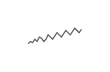
\begin{tikzpicture}[x=0.08em, y=0.08em, line width=0.4pt]
                \draw[FooterGray] (0,3) -- (1,4) -- (2,3.5) -- (3,5) -- (4,4) -- (5,6) -- (6,5.5) -- (7,4) -- (8,5) -- (9,7) -- (10,6) -- (11,5) -- (12,6.5) -- (13,8) -- (14,7) -- (15,6) -- (16,7.5) -- (17,9) -- (18,8) -- (19,7) -- (20,8.5) -- (21,10) -- (22,9) -- (23,8) -- (24,9.5);
            \end{tikzpicture}%
        }%
        \hskip0.5cm%
    }%
    \vskip6pt%
}

%=============================================================================
% PACKAGES
%=============================================================================
\usepackage[utf8]{inputenc}
\DeclareUnicodeCharacter{03B1}{\ensuremath{\alpha}}
\usepackage[T1]{fontenc}
\usepackage{amsmath, amssymb, amsthm}
\usepackage{mathtools}
\usepackage{bm}
\usepackage{tikz}
\usetikzlibrary{arrows.meta, positioning, shapes, calc, decorations.pathreplacing, shadings}
\usepackage{booktabs}
\usepackage{multirow}
\usepackage{array}
\usepackage{graphicx}
\usepackage{animate}
\usepackage{hyperref}
\usepackage{colortbl}
\usepackage{listings}
\lstset{language=Python, basicstyle=\ttfamily\scriptsize, keywordstyle=\color{MainBlue}\bfseries,
  commentstyle=\color{Forest}, stringstyle=\color{Crimson}, breaklines=true,
  frame=none, backgroundcolor=\color{VeryLightGray}, xleftmargin=2mm}
\hypersetup{colorlinks=true, linkcolor=MainBlue, urlcolor=MainBlue}
\graphicspath{{../../logos/}{../../charts/}{../../photos/}}
\usepackage{xcolor}
\hfuzz=2pt  % Suppress tiny overfull warnings (<2pt)
\vfuzz=2pt  % Suppress tiny vertical overfull warnings (<2pt)
% \mathrm in the sans-serif family of the slides (beamer resets \mathrm to the serif family at \begin{document};
% this hook runs after beamer's, so WN, Var, RMSE, ... in formulas match the surrounding text)
% Bold vectors and matrices in the same sans-serif family: \mathbf{A} in sans bold (beamer's own \mathbf came out in
% medium weight), and the bold upright Greek capitals of \boldsymbol / \bm (\bSigma, \bPhi, \boldsymbol{\Theta}) in
% cmss bold: bm.sty fixes its "boldoperators" font when it is loaded (serif cmbx), before beamer switches the
% operators to cmss, so it is reset here.
\AtBeginDocument{%
  \SetMathAlphabet{\mathrm}{normal}{\encodingdefault}{\sfdefault}{\mddefault}{n}%
  \SetMathAlphabet{\mathrm}{bold}{\encodingdefault}{\sfdefault}{bx}{n}%
  \SetMathAlphabet{\mathbf}{normal}{\encodingdefault}{\sfdefault}{bx}{n}%
  \SetMathAlphabet{\mathbf}{bold}{\encodingdefault}{\sfdefault}{bx}{n}%
  \SetSymbolFont{boldoperators}{normal}{OT1}{cmss}{bx}{n}%
  \SetSymbolFont{boldoperators}{bold}{OT1}{cmss}{bx}{n}}

%=============================================================================
% QUANTLET COMMANDS
%   \quantlet{<displayed name>}{<url>}       (generic, compatible with the older TSA decks)
%   \tsaquantlet{Ch_05}{TSA_ch5_garch}       -> https://github.com/danpele/Time-Series-Analysis/tree/main/Quantlets/Ch_05/TSA_ch5_garch
%   \qlurl{<folder>} is defined per chapter by the generator (Quantlets/Ch_NN/<folder>)
%=============================================================================
\newcommand{\tsarepo}{https://github.com/danpele/Time-Series-Analysis}
\newcommand{\tsaqlbase}{https://github.com/danpele/Time-Series-Analysis/tree/main/Quantlets}
\newcommand{\quantlet}[2]{%
    \hfill\href{#2}{%
        \raisebox{-0.15em}{
\includegraphics[height=0.7em]{ql_logo.png}}%
        \textcolor{MainBlue}{\tiny\ #1}%
    }%
}
\newcommand{\tsaquantlet}[2]{\quantlet{\detokenize{#2}}{\tsaqlbase/#1/#2}}

%=============================================================================
% NOTEBOOKS (Google Colab)
%   \colaburl{notebooks/EN/chapter5_seminar_notebook.ipynb} -> the Colab link of a file in the TSA repo
%   \nb: the chapter notebook (each seminar deck redefines it with \renewcommand)
%=============================================================================
\newcommand{\colaburl}[1]{https://colab.research.google.com/github/danpele/Time-Series-Analysis/blob/main/#1}
\newcommand{\nb}{https://colab.research.google.com/github/danpele/Time-Series-Analysis/tree/main/notebooks/EN}
\newcommand{\nbname}{notebooks/EN}

%=============================================================================
% SLIDE HELPERS (used by the generators; the same as in MFM)
%=============================================================================
% local font size for list bodies (the preamble forces \normalsize)
\newcommand{\itemsize}[1]{\setbeamertemplate{itemize/enumerate body begin}{#1}\setbeamertemplate{itemize/enumerate subbody begin}{#1}}
\newcommand{\intitle}[1]{{\hypersetup{urlcolor=white}#1}}   % white links inside coloured title bars
\newcommand{\imgcap}[1]{{\scriptsize #1}\\[0.5mm]}          % caption under a photo
\newcommand{\imgcredit}[2]{{\tiny\color{FooterGray}\href{#1}{#2}}}   % image credit: source URL, author/licence
\newcommand{\aiprompt}[1]{{\ttfamily\color{MainBlue}#1}}     % a prompt to an AI assistant

%=============================================================================
% SEMINARS: student version by default; the instructor wrapper *_solutions.tex sets \solutionstrue
%=============================================================================
\makeatletter\@ifundefined{ifsolutions}{\expandafter\newif\csname ifsolutions\endcsname}{}\makeatother
\newcommand{\solonly}[1]{\ifsolutions #1\fi}
\newcommand{\propsub}{\ifsolutions\else\framesubtitle{\ifdefined\tsalang Rezolvarea se discută la seminar\else Solution discussed in class\fi}\fi}

%=============================================================================
% APPENDIX AND CHAPTER LINKS (latex/appendix_links.py writes the calls; it also re-declares these
% macros before \begin{document}, so the decks compile with or without this preamble block)
%=============================================================================
\providecommand{\tsaapplink}[3]{\hypertarget{#2}{}\hyperlink{#1}{\beamergotobutton{#3}}}
\providecommand{\tsaappback}[2]{\begin{tikzpicture}[remember picture,overlay]\node[anchor=south east] at ([xshift=-3mm,yshift=7mm]current page.south east){\hyperlink{#1}{\beamerreturnbutton{#2}}};\end{tikzpicture}}
\providecommand{\tsachlink}[2]{\href{#1}{#2}}
\providecommand{\tsachlinkt}[2]{\href{#1}{\usebeamercolor[fg]{frametitle}#2}}

%=============================================================================
% QUANTINAR COMMAND: link către un curs Quantinar (subiecte avansate)
%=============================================================================
\newcommand{\quantinar}[2]{%
    \href{#2}{%
        \raisebox{-0.15em}{
\includegraphics[height=0.8em]{qr_logo.png}}%
        \textcolor{MainBlue}{\scriptsize\ #1}%
    }%
}

%=============================================================================
% CUSTOM TITLE PAGE
%=============================================================================
\defbeamertemplate*{title page}{hybrid}[1][]
{
    \vspace{0.2cm}
    % Logos row - top header (with clickable links)
    \begin{center}
        \href{https://www.ase.ro}{
\includegraphics[height=1.0cm]{ase_logo.png}}\hspace{0.3cm}%
        \href{https://theida.net}{
\includegraphics[height=1.0cm]{ida_logo.png}}\hspace{0.3cm}%
        \href{https://blockchain-research-center.com}{
\includegraphics[height=1.0cm]{brc_logo.png}}\hspace{0.3cm}%
        \href{https://www.ai4efin.ase.ro}{
\includegraphics[height=1.0cm]{ai4efin_logo.png}}\hspace{0.3cm}%
        \href{https://ipe.ro/new}{
\includegraphics[height=1.0cm]{acad_logo.png}}\hspace{0.3cm}%
        \href{https://www.digital-finance-msca.com}{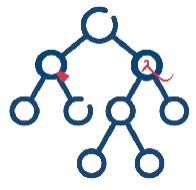
\includegraphics[height=1.0cm]{msca_logo.png}}%
    \end{center}

    \vspace{0.6cm}

    % Main title with Q logos on sides (with clickable links)
    \begin{center}
        \begin{minipage}{0.1\textwidth}
            \centering
            \href{https://quantlet.com}{
\includegraphics[height=1.1cm]{ql_logo.png}}
        \end{minipage}%
        \begin{minipage}{0.78\textwidth}
            \centering
            {\LARGE\bfseries\usebeamercolor[fg]{title}\inserttitle}

            \vspace{0.3cm}

            {\usebeamerfont{subtitle}\usebeamercolor[fg]{title}\insertsubtitle}
        \end{minipage}%
        \begin{minipage}{0.1\textwidth}
            \centering
            \href{https://quantinar.com}{
\includegraphics[height=1.1cm]{qr_logo.png}}
        \end{minipage}
    \end{center}

    \vspace{0.6cm}

    % Authors (left aligned)
    \hspace{0.5cm}{\usebeamerfont{author}\insertauthor}

    \vspace{0.3cm}

    % Institute/Affiliations (left aligned)
    \hspace{0.5cm}\begin{minipage}[t]{0.9\textwidth}
        \raggedright\small\insertinstitute
    \end{minipage}
}

%=============================================================================
% THEOREM ENVIRONMENTS
%=============================================================================
\theoremstyle{definition}
\setbeamertemplate{theorems}[numbered]
\ifdefined\tsalang
\newtheorem{defn}{Definiție}
\newtheorem{thm}{Teoremă}
\newtheorem{prop}{Propoziție}
\newtheorem{rmk}{Observație}
\else
\newtheorem{defn}{Definition}
\newtheorem{thm}{Theorem}
\newtheorem{prop}{Proposition}
\newtheorem{rmk}{Remark}
\fi

%=============================================================================
% CENTRED MINIPAGE (no extra vertical space)
%=============================================================================
\newenvironment{cminipage}[1]{%
    \par\noindent\hfill\begin{minipage}{#1}\ignorespaces
}{%
    \end{minipage}\hfill\null\par
}

%=============================================================================
% CUSTOM COMMANDS
%=============================================================================
\newcommand{\E}{\mathbb{E}}
\newcommand{\Var}{\text{Var}}
\newcommand{\Cov}{\text{Cov}}
\newcommand{\Corr}{\text{Corr}}
\newcommand{\R}{\mathbb{R}}
\newcommand{\N}{\mathbb{N}}
\newcommand{\Z}{\mathbb{Z}}
\newcommand{\B}{\mathbf{B}}
\newcommand{\imark}{\textcolor{MainBlue}{\textbullet}}
\newcommand{\RMSE}{\text{RMSE}}
\newcommand{\MAE}{\text{MAE}}
\newcommand{\MAPE}{\text{MAPE}}

% Boldface vector/matrix commands (VAR, VECM, state space; also used by the older TSA decks)
\newcommand{\bY}{\mathbf{Y}}
\newcommand{\bX}{\mathbf{X}}
\newcommand{\bA}{\mathbf{A}}
\newcommand{\bB}{\mathbf{B}}
\newcommand{\bepsilon}{\boldsymbol{\varepsilon}}
\newcommand{\bSigma}{\boldsymbol{\Sigma}}
\newcommand{\bPhi}{\boldsymbol{\Phi}}
\newcommand{\bGamma}{\boldsymbol{\Gamma}}
\newcommand{\bPi}{\boldsymbol{\Pi}}
\newcommand{\bc}{\mathbf{c}}
\newcommand{\balpha}{\boldsymbol{\alpha}}
\newcommand{\bbeta}{\boldsymbol{\beta}}
\newcommand{\bvarepsilon}{\boldsymbol{\varepsilon}}

% Legacy seminar marks (older TSA seminar decks)
\newcommand{\correct}{\textcolor{Forest}{\checkmark}}
\newcommand{\incorrect}{\textcolor{Crimson}{\texttimes}}
 se definește
%   \newcommand{\coursename}{Time Series Analysis}      (EN)
%   \newcommand{\coursename}{Serii de timp}       (RO)  și  \def\tsalang{ro}
% Fișierele .tex se află în EN/Courses, EN/Seminars, RO/Cursuri, RO/Seminarii (două niveluri sub rădăcină).
% Deck-urile sînt generate de latex/build_chapterN.py / build_seminarN.py (vezi latex/tsa_build.py).

\documentclass[9pt, aspectratio=169, t]{beamer}
\providecommand{\coursename}{Time Series Analysis}

% Ensure content fits on slides
\setbeamersize{text margin left=8mm, text margin right=8mm}
% Smaller institute font (title page)
\setbeamerfont{institute}{size=\footnotesize}

%=============================================================================
% THEME AND STYLE CONFIGURATION
%=============================================================================
\usetheme{default}
% Using default theme for clean header/footer control

% Color Palette (matching Redispatch PDF)
\definecolor{MainBlue}{RGB}{26, 58, 110}
\definecolor{AccentBlue}{RGB}{26, 58, 110}
\definecolor{IDAred}{RGB}{205, 0, 0}
\definecolor{DarkGray}{RGB}{51, 51, 51}
\definecolor{MediumGray}{RGB}{128, 128, 128}
\definecolor{LightGray}{RGB}{248, 248, 248}
\definecolor{VeryLightGray}{RGB}{235, 235, 235}
\definecolor{KeynoteGray}{RGB}{218, 218, 218}
\definecolor{SectionGray}{RGB}{120, 120, 120}
\definecolor{FooterGray}{RGB}{100, 100, 100}
\definecolor{Crimson}{RGB}{220, 53, 69}
\definecolor{Forest}{RGB}{46, 125, 50}
\definecolor{Amber}{RGB}{181, 133, 63}
\definecolor{Orange}{RGB}{230, 126, 34}
\definecolor{Purple}{RGB}{142, 68, 173}

% Gradient background (exact Keynote 315° gradient: white to RGB 218,218,218)
\setbeamertemplate{background}{%
    \begin{tikzpicture}[remember picture, overlay]
        \shade[shading=axis, shading angle=315,
        top color=white, bottom color=KeynoteGray]
        (current page.south west) rectangle (current page.north east);
    \end{tikzpicture}%
}
% Fallback solid color for compatibility
\setbeamercolor{background canvas}{bg=}

\setbeamercolor{palette primary}{bg=MainBlue, fg=white}
\setbeamercolor{palette secondary}{bg=MainBlue!85, fg=white}
\setbeamercolor{palette tertiary}{bg=MainBlue!70, fg=white}
\setbeamercolor{structure}{fg=MainBlue}
\setbeamercolor{title}{fg=IDAred}
\setbeamercolor{frametitle}{fg=IDAred, bg=}
\setbeamercolor{block title}{bg=MainBlue, fg=white}
\setbeamercolor{block body}{bg=VeryLightGray, fg=DarkGray}
\setbeamercolor{block title alerted}{bg=Crimson, fg=white}
\setbeamercolor{block body alerted}{bg=Crimson!8, fg=DarkGray}
\setbeamercolor{block title example}{bg=Forest, fg=white}
\setbeamercolor{block body example}{bg=Forest!8, fg=DarkGray}
\setbeamercolor{item}{fg=MainBlue}

% Footer colors (override Madrid theme blue)
\setbeamercolor{author in head/foot}{fg=FooterGray, bg=}
\setbeamercolor{title in head/foot}{fg=FooterGray, bg=}
\setbeamercolor{date in head/foot}{fg=FooterGray, bg=}
\setbeamercolor{section in head/foot}{fg=FooterGray, bg=}
\setbeamercolor{subsection in head/foot}{fg=FooterGray, bg=}

% Bullet styles (apply everywhere including blocks)
\setbeamertemplate{itemize item}{\color{MainBlue}$\boxdot$}
\setbeamertemplate{itemize subitem}{\color{MainBlue}$\blacktriangleright$}
\setbeamertemplate{itemize subsubitem}{\color{MainBlue}\tiny$\bullet$}
\setbeamertemplate{itemize/enumerate body begin}{\normalsize}
\setbeamertemplate{itemize/enumerate subbody begin}{\normalsize}

% Item spacing - compact style
\setlength{\leftmargini}{10pt}       % Level 1: minimal indent
\setlength{\leftmarginii}{10pt}      % Level 2: minimal additional indent
% Compact list spacing (zero extra space before/after lists in blocks)
\makeatletter
\def\@listi{\leftmargin\leftmargini \topsep 0pt \parsep 0pt \itemsep 0pt}
\def\@listii{\leftmargin\leftmarginii \topsep 0pt \parsep 0pt \itemsep 0pt}
\makeatother

\setbeamertemplate{navigation symbols}{}

%=============================================================================
% CUSTOM HEADLINE
%=============================================================================
\setbeamertemplate{headline}{%
    \vskip10pt%
    \hbox to \paperwidth{%
        \hskip0.5cm%
        {\small\color{FooterGray}\renewcommand{\hyperlink}[2]{##2}\insertsectionhead}%
        \hfill%
        \textcolor{FooterGray}{\small\insertframenumber}%
        \hskip0.5cm%
    }%
    \vskip4pt%
    {\color{FooterGray}\hrule height 0.4pt}%
}

%=============================================================================
% CUSTOM FOOTER
%=============================================================================
\usepackage{fontawesome5}

\setbeamertemplate{footline}{%
    {\color{FooterGray}\hrule height 0.4pt}%
    \vskip4pt%
    \hbox to \paperwidth{%
        \hskip0.5cm%
        \textcolor{FooterGray}{\small\coursename}%
        \hfill%
        \raisebox{-0.1em}{%
            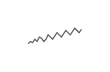
\begin{tikzpicture}[x=0.08em, y=0.08em, line width=0.4pt]
                \draw[FooterGray] (0,3) -- (1,4) -- (2,3.5) -- (3,5) -- (4,4) -- (5,6) -- (6,5.5) -- (7,4) -- (8,5) -- (9,7) -- (10,6) -- (11,5) -- (12,6.5) -- (13,8) -- (14,7) -- (15,6) -- (16,7.5) -- (17,9) -- (18,8) -- (19,7) -- (20,8.5) -- (21,10) -- (22,9) -- (23,8) -- (24,9.5);
            \end{tikzpicture}%
        }%
        \hskip0.5cm%
    }%
    \vskip6pt%
}

%=============================================================================
% PACKAGES
%=============================================================================
\usepackage[utf8]{inputenc}
\DeclareUnicodeCharacter{03B1}{\ensuremath{\alpha}}
\usepackage[T1]{fontenc}
\usepackage{amsmath, amssymb, amsthm}
\usepackage{mathtools}
\usepackage{bm}
\usepackage{tikz}
\usetikzlibrary{arrows.meta, positioning, shapes, calc, decorations.pathreplacing, shadings}
\usepackage{booktabs}
\usepackage{multirow}
\usepackage{array}
\usepackage{graphicx}
\usepackage{animate}
\usepackage{hyperref}
\usepackage{colortbl}
\usepackage{listings}
\lstset{language=Python, basicstyle=\ttfamily\scriptsize, keywordstyle=\color{MainBlue}\bfseries,
  commentstyle=\color{Forest}, stringstyle=\color{Crimson}, breaklines=true,
  frame=none, backgroundcolor=\color{VeryLightGray}, xleftmargin=2mm}
\hypersetup{colorlinks=true, linkcolor=MainBlue, urlcolor=MainBlue}
\graphicspath{{../../logos/}{../../charts/}{../../photos/}}
\usepackage{xcolor}
\hfuzz=2pt  % Suppress tiny overfull warnings (<2pt)
\vfuzz=2pt  % Suppress tiny vertical overfull warnings (<2pt)
% \mathrm in the sans-serif family of the slides (beamer resets \mathrm to the serif family at \begin{document};
% this hook runs after beamer's, so WN, Var, RMSE, ... in formulas match the surrounding text)
% Bold vectors and matrices in the same sans-serif family: \mathbf{A} in sans bold (beamer's own \mathbf came out in
% medium weight), and the bold upright Greek capitals of \boldsymbol / \bm (\bSigma, \bPhi, \boldsymbol{\Theta}) in
% cmss bold: bm.sty fixes its "boldoperators" font when it is loaded (serif cmbx), before beamer switches the
% operators to cmss, so it is reset here.
\AtBeginDocument{%
  \SetMathAlphabet{\mathrm}{normal}{\encodingdefault}{\sfdefault}{\mddefault}{n}%
  \SetMathAlphabet{\mathrm}{bold}{\encodingdefault}{\sfdefault}{bx}{n}%
  \SetMathAlphabet{\mathbf}{normal}{\encodingdefault}{\sfdefault}{bx}{n}%
  \SetMathAlphabet{\mathbf}{bold}{\encodingdefault}{\sfdefault}{bx}{n}%
  \SetSymbolFont{boldoperators}{normal}{OT1}{cmss}{bx}{n}%
  \SetSymbolFont{boldoperators}{bold}{OT1}{cmss}{bx}{n}}

%=============================================================================
% QUANTLET COMMANDS
%   \quantlet{<displayed name>}{<url>}       (generic, compatible with the older TSA decks)
%   \tsaquantlet{Ch_05}{TSA_ch5_garch}       -> https://github.com/danpele/Time-Series-Analysis/tree/main/Quantlets/Ch_05/TSA_ch5_garch
%   \qlurl{<folder>} is defined per chapter by the generator (Quantlets/Ch_NN/<folder>)
%=============================================================================
\newcommand{\tsarepo}{https://github.com/danpele/Time-Series-Analysis}
\newcommand{\tsaqlbase}{https://github.com/danpele/Time-Series-Analysis/tree/main/Quantlets}
\newcommand{\quantlet}[2]{%
    \hfill\href{#2}{%
        \raisebox{-0.15em}{
\includegraphics[height=0.7em]{ql_logo.png}}%
        \textcolor{MainBlue}{\tiny\ #1}%
    }%
}
\newcommand{\tsaquantlet}[2]{\quantlet{\detokenize{#2}}{\tsaqlbase/#1/#2}}

%=============================================================================
% NOTEBOOKS (Google Colab)
%   \colaburl{notebooks/EN/chapter5_seminar_notebook.ipynb} -> the Colab link of a file in the TSA repo
%   \nb: the chapter notebook (each seminar deck redefines it with \renewcommand)
%=============================================================================
\newcommand{\colaburl}[1]{https://colab.research.google.com/github/danpele/Time-Series-Analysis/blob/main/#1}
\newcommand{\nb}{https://colab.research.google.com/github/danpele/Time-Series-Analysis/tree/main/notebooks/EN}
\newcommand{\nbname}{notebooks/EN}

%=============================================================================
% SLIDE HELPERS (used by the generators; the same as in MFM)
%=============================================================================
% local font size for list bodies (the preamble forces \normalsize)
\newcommand{\itemsize}[1]{\setbeamertemplate{itemize/enumerate body begin}{#1}\setbeamertemplate{itemize/enumerate subbody begin}{#1}}
\newcommand{\intitle}[1]{{\hypersetup{urlcolor=white}#1}}   % white links inside coloured title bars
\newcommand{\imgcap}[1]{{\scriptsize #1}\\[0.5mm]}          % caption under a photo
\newcommand{\imgcredit}[2]{{\tiny\color{FooterGray}\href{#1}{#2}}}   % image credit: source URL, author/licence
\newcommand{\aiprompt}[1]{{\ttfamily\color{MainBlue}#1}}     % a prompt to an AI assistant

%=============================================================================
% SEMINARS: student version by default; the instructor wrapper *_solutions.tex sets \solutionstrue
%=============================================================================
\makeatletter\@ifundefined{ifsolutions}{\expandafter\newif\csname ifsolutions\endcsname}{}\makeatother
\newcommand{\solonly}[1]{\ifsolutions #1\fi}
\newcommand{\propsub}{\ifsolutions\else\framesubtitle{\ifdefined\tsalang Rezolvarea se discută la seminar\else Solution discussed in class\fi}\fi}

%=============================================================================
% APPENDIX AND CHAPTER LINKS (latex/appendix_links.py writes the calls; it also re-declares these
% macros before \begin{document}, so the decks compile with or without this preamble block)
%=============================================================================
\providecommand{\tsaapplink}[3]{\hypertarget{#2}{}\hyperlink{#1}{\beamergotobutton{#3}}}
\providecommand{\tsaappback}[2]{\begin{tikzpicture}[remember picture,overlay]\node[anchor=south east] at ([xshift=-3mm,yshift=7mm]current page.south east){\hyperlink{#1}{\beamerreturnbutton{#2}}};\end{tikzpicture}}
\providecommand{\tsachlink}[2]{\href{#1}{#2}}
\providecommand{\tsachlinkt}[2]{\href{#1}{\usebeamercolor[fg]{frametitle}#2}}

%=============================================================================
% QUANTINAR COMMAND: link către un curs Quantinar (subiecte avansate)
%=============================================================================
\newcommand{\quantinar}[2]{%
    \href{#2}{%
        \raisebox{-0.15em}{
\includegraphics[height=0.8em]{qr_logo.png}}%
        \textcolor{MainBlue}{\scriptsize\ #1}%
    }%
}

%=============================================================================
% CUSTOM TITLE PAGE
%=============================================================================
\defbeamertemplate*{title page}{hybrid}[1][]
{
    \vspace{0.2cm}
    % Logos row - top header (with clickable links)
    \begin{center}
        \href{https://www.ase.ro}{
\includegraphics[height=1.0cm]{ase_logo.png}}\hspace{0.3cm}%
        \href{https://theida.net}{
\includegraphics[height=1.0cm]{ida_logo.png}}\hspace{0.3cm}%
        \href{https://blockchain-research-center.com}{
\includegraphics[height=1.0cm]{brc_logo.png}}\hspace{0.3cm}%
        \href{https://www.ai4efin.ase.ro}{
\includegraphics[height=1.0cm]{ai4efin_logo.png}}\hspace{0.3cm}%
        \href{https://ipe.ro/new}{
\includegraphics[height=1.0cm]{acad_logo.png}}\hspace{0.3cm}%
        \href{https://www.digital-finance-msca.com}{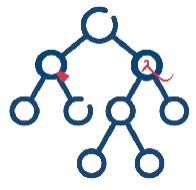
\includegraphics[height=1.0cm]{msca_logo.png}}%
    \end{center}

    \vspace{0.6cm}

    % Main title with Q logos on sides (with clickable links)
    \begin{center}
        \begin{minipage}{0.1\textwidth}
            \centering
            \href{https://quantlet.com}{
\includegraphics[height=1.1cm]{ql_logo.png}}
        \end{minipage}%
        \begin{minipage}{0.78\textwidth}
            \centering
            {\LARGE\bfseries\usebeamercolor[fg]{title}\inserttitle}

            \vspace{0.3cm}

            {\usebeamerfont{subtitle}\usebeamercolor[fg]{title}\insertsubtitle}
        \end{minipage}%
        \begin{minipage}{0.1\textwidth}
            \centering
            \href{https://quantinar.com}{
\includegraphics[height=1.1cm]{qr_logo.png}}
        \end{minipage}
    \end{center}

    \vspace{0.6cm}

    % Authors (left aligned)
    \hspace{0.5cm}{\usebeamerfont{author}\insertauthor}

    \vspace{0.3cm}

    % Institute/Affiliations (left aligned)
    \hspace{0.5cm}\begin{minipage}[t]{0.9\textwidth}
        \raggedright\small\insertinstitute
    \end{minipage}
}

%=============================================================================
% THEOREM ENVIRONMENTS
%=============================================================================
\theoremstyle{definition}
\setbeamertemplate{theorems}[numbered]
\ifdefined\tsalang
\newtheorem{defn}{Definiție}
\newtheorem{thm}{Teoremă}
\newtheorem{prop}{Propoziție}
\newtheorem{rmk}{Observație}
\else
\newtheorem{defn}{Definition}
\newtheorem{thm}{Theorem}
\newtheorem{prop}{Proposition}
\newtheorem{rmk}{Remark}
\fi

%=============================================================================
% CENTRED MINIPAGE (no extra vertical space)
%=============================================================================
\newenvironment{cminipage}[1]{%
    \par\noindent\hfill\begin{minipage}{#1}\ignorespaces
}{%
    \end{minipage}\hfill\null\par
}

%=============================================================================
% CUSTOM COMMANDS
%=============================================================================
\newcommand{\E}{\mathbb{E}}
\newcommand{\Var}{\text{Var}}
\newcommand{\Cov}{\text{Cov}}
\newcommand{\Corr}{\text{Corr}}
\newcommand{\R}{\mathbb{R}}
\newcommand{\N}{\mathbb{N}}
\newcommand{\Z}{\mathbb{Z}}
\newcommand{\B}{\mathbf{B}}
\newcommand{\imark}{\textcolor{MainBlue}{\textbullet}}
\newcommand{\RMSE}{\text{RMSE}}
\newcommand{\MAE}{\text{MAE}}
\newcommand{\MAPE}{\text{MAPE}}

% Boldface vector/matrix commands (VAR, VECM, state space; also used by the older TSA decks)
\newcommand{\bY}{\mathbf{Y}}
\newcommand{\bX}{\mathbf{X}}
\newcommand{\bA}{\mathbf{A}}
\newcommand{\bB}{\mathbf{B}}
\newcommand{\bepsilon}{\boldsymbol{\varepsilon}}
\newcommand{\bSigma}{\boldsymbol{\Sigma}}
\newcommand{\bPhi}{\boldsymbol{\Phi}}
\newcommand{\bGamma}{\boldsymbol{\Gamma}}
\newcommand{\bPi}{\boldsymbol{\Pi}}
\newcommand{\bc}{\mathbf{c}}
\newcommand{\balpha}{\boldsymbol{\alpha}}
\newcommand{\bbeta}{\boldsymbol{\beta}}
\newcommand{\bvarepsilon}{\boldsymbol{\varepsilon}}

% Legacy seminar marks (older TSA seminar decks)
\newcommand{\correct}{\textcolor{Forest}{\checkmark}}
\newcommand{\incorrect}{\textcolor{Crimson}{\texttimes}}


\newcommand{\qlurl}[1]{https://github.com/danpele/Time-Series-Analysis/tree/main/Quantlets/Ch_07/#1}

% Clickable citations (DOIs verified via Crossref)
\newcommand{\refHP}{\href{https://doi.org/10.1007/978-3-031-13584-2}{Huang și Petukhina (2022)}}
\newcommand{\refHamilton}{\href{https://doi.org/10.2307/j.ctv14jx6sm}{Hamilton (1994)}}
\newcommand{\refLut}{\href{https://doi.org/10.1007/978-3-540-27752-1}{Lütkepohl (2005)}}
\newcommand{\refJohBook}{\href{https://doi.org/10.1093/0198774508.001.0001}{Johansen (1995)}}
\newcommand{\refJus}{\href{https://doi.org/10.1093/oso/9780199285662.001.0001}{Juselius (2006)}}
\newcommand{\refEG}{\href{https://doi.org/10.2307/1913236}{Engle și Granger (1987)}}
\newcommand{\refGranger}{\href{https://doi.org/10.1016/0304-4076(81)90079-8}{Granger (1981)}}
\newcommand{\refGrangerN}{\href{https://doi.org/10.1257/0002828041464669}{Granger (2004)}}
\newcommand{\refGN}{\href{https://doi.org/10.1016/0304-4076(74)90034-7}{Granger și Newbold (1974)}}
\newcommand{\refMurray}{\href{https://doi.org/10.1080/00031305.1994.10476017}{Murray (1994)}}
\newcommand{\refPO}{\href{https://doi.org/10.2307/2938339}{Phillips și Ouliaris (1990)}}
\newcommand{\refMacKinnon}{\href{https://doi.org/10.1080/07350015.1994.10510005}{MacKinnon (1994)}}
\newcommand{\refMacKinnonb}{\href{https://ideas.repec.org/p/qed/wpaper/1227.html}{MacKinnon (2010)}}
\newcommand{\refSW}{\href{https://doi.org/10.1080/01621459.1988.10478707}{Stock și Watson (1988)}}
\newcommand{\refSWd}{\href{https://doi.org/10.2307/2951763}{Stock și Watson (1993)}}
\newcommand{\refDHSY}{\href{https://doi.org/10.2307/2231972}{Davidson et al.\ (1978)}}
\newcommand{\refBDM}{\href{https://doi.org/10.1111/1467-9892.00091}{Banerjee, Dolado și Mestre (1998)}}
\newcommand{\refJohA}{\href{https://doi.org/10.1016/0165-1889(88)90041-3}{Johansen (1988)}}
\newcommand{\refJohB}{\href{https://doi.org/10.2307/2938278}{Johansen (1991)}}
\newcommand{\refJJ}{\href{https://doi.org/10.1111/j.1468-0084.1990.mp52002003.x}{Johansen și Juselius (1990)}}
\newcommand{\refOL}{\href{https://doi.org/10.1111/j.1468-0084.1992.tb00013.x}{Osterwald-Lenum (1992)}}
\newcommand{\refMHM}{\href{https://doi.org/10.1002/(SICI)1099-1255(199909/10)14:5<563::AID-JAE530>3.0.CO;2-R}{MacKinnon, Haug și Michelis (1999)}}
\newcommand{\refRA}{\href{https://doi.org/10.1111/j.1467-9892.1992.tb00113.x}{Reinsel și Ahn (1992)}}
\newcommand{\refEY}{\href{https://doi.org/10.1016/0304-4076(87)90085-6}{Engle și Yoo (1987)}}
\newcommand{\refCD}{\href{https://doi.org/10.1080/07350015.1998.10524784}{Christoffersen și Diebold (1998)}}
\newcommand{\refCS}{\href{https://doi.org/10.1086/261502}{Campbell și Shiller (1987)}}
\newcommand{\refBalassa}{\href{https://doi.org/10.1086/258965}{Balassa (1964)}}
\newcommand{\refTT}{\href{https://doi.org/10.1257/0895330042632744}{Taylor și Taylor (2004)}}
\newcommand{\refGGR}{\href{https://doi.org/10.1093/rfs/hhj020}{Gatev, Goetzmann și Rouwenhorst (2006)}}
\newcommand{\refDoFaff}{\href{https://doi.org/10.2469/faj.v66.n4.1}{Do și Faff (2010)}}

\title[Serii de timp]{Serii de timp}
\subtitle{Capitolul 7: Cointegrare și VECM}
\author[D.T. Pele]{Daniel Traian PELE}
\institute{Academia de Studii Economice din București\\
IDA Institute Digital Assets\\
Blockchain Research Center\\
AI4EFin Artificial Intelligence for Energy Finance\\
Academia Română, Institutul de Prognoză Economică\\
MSCA Digital Finance}
\date{}

%=============================================================================
\providecommand{\tsaapplink}[3]{\hypertarget{#2}{}\hyperlink{#1}{\beamergotobutton{#3}}}  % APPLINKS-MACROS
\providecommand{\tsaappback}[2]{\begin{tikzpicture}[remember picture,overlay]\node[anchor=south east] at ([xshift=-3mm,yshift=7mm]current page.south east){\hyperlink{#1}{\beamerreturnbutton{#2}}};\end{tikzpicture}}  % APPLINKS-MACROS
\providecommand{\tsachlink}[2]{\href{#1}{#2}}  % APPLINKS-MACROS
\providecommand{\tsachlinkt}[2]{\href{#1}{\usebeamercolor[fg]{frametitle}#2}}  % APPLINKS-MACROS
\begin{document}
%=============================================================================

{
\setbeamertemplate{headline}{}
\setbeamertemplate{footline}{}
\begin{frame}[noframenumbering]
    \titlepage
\end{frame}
}
% BEGIN-ACRONYMS (generat de latex/acronyms.py; nu editati manual)
\begin{frame}{Acronime folosite în acest material (1/2)}
\setbeamertemplate{itemize/enumerate body begin}{\tiny}
\begin{columns}[T]
\begin{column}{0.49\textwidth}
\begin{itemize}\setlength{\itemsep}{0pt}
    \item \textbf{ACF}: Autocorrelation Function (funcția de autocorelație)
    \item \textbf{ADF}: Augmented Dickey–Fuller (test) — testul Dickey–Fuller augmentat
    \item \textbf{AI}: Artificial Intelligence (inteligență artificială)
    \item \textbf{AIC}: Akaike Information Criterion (criteriul informațional Akaike)
    \item \textbf{AR}: AutoRegressive (model); in event studies: Abnormal Return (model autoregresiv; în studiile de eveniment: randament anormal)
    \item \textbf{ARCH}: AutoRegressive Conditional Heteroskedasticity (heteroscedasticitate condiționată autoregresivă)
    \item \textbf{ARFIMA}: AutoRegressive Fractionally Integrated Moving Average (model) — model autoregresiv fracționar integrat cu medie mobilă
    \item \textbf{BAC}: Bank of America (NYSE ticker) — Bank of America (simbolul la NYSE)
    \item \textbf{BIC}: Bayesian Information Criterion (criteriul informațional bayesian (Schwarz))
    \item \textbf{BNR}: Banca Națională a României
    \item \textbf{BVB}: Bursa de Valori București
    \item \textbf{DHSY}: Davidson, Hendry, Srba and Yeo (1978) — modelul de consum cu corecția erorii al lui Davidson, Hendry, Srba și Yeo (1978)
    \item \textbf{DOLS}: Dynamic Ordinary Least Squares (metoda celor mai mici pătrate dinamică)
\end{itemize}
\end{column}
\begin{column}{0.49\textwidth}
\begin{itemize}\setlength{\itemsep}{0pt}
    \item \textbf{DW}: Durbin–Watson (statistic) — statistica Durbin–Watson
    \item \textbf{ECM}: Error Correction Model (model cu corecția erorii)
    \item \textbf{FRED}: Federal Reserve Economic Data (baza de date economice a Rezervei Federale din St. Louis)
    \item \textbf{GS}: Goldman Sachs (NYSE ticker) — Goldman Sachs (simbolul la NYSE)
    \item \textbf{GS1}: 1-year Treasury constant-maturity yield (FRED series code) — codul FRED al randamentului titlurilor de stat americane la 1 an
    \item \textbf{GS10}: 10-year Treasury constant-maturity yield (FRED series code) — codul FRED al randamentului titlurilor de stat americane la 10 ani
    \item \textbf{GS5}: 5-year Treasury constant-maturity yield (FRED series code) — codul FRED al randamentului titlurilor de stat americane la 5 ani
    \item \textbf{IAPC}: Indicele armonizat al prețurilor de consum
    \item \textbf{JPM}: JPMorgan Chase (NYSE ticker) — JPMorgan Chase (simbolul la NYSE)
    \item \textbf{LR}: Likelihood Ratio (test) — testul raportului de verosimilitate
    \item \textbf{MS}: Morgan Stanley (NYSE ticker) — Morgan Stanley (simbolul la NYSE)
    \item \textbf{OLS}: Ordinary Least Squares (metoda celor mai mici pătrate)
    \item \textbf{PIB}: Produsul intern brut
\end{itemize}
\end{column}
\end{columns}
\end{frame}
\begin{frame}{Acronime folosite în acest material (2/2)}
\setbeamertemplate{itemize/enumerate body begin}{\tiny}
\begin{columns}[T]
\begin{column}{0.49\textwidth}
\begin{itemize}\setlength{\itemsep}{0pt}
    \item \textbf{PPP}: Purchasing Power Parity (paritatea puterii de cumpărare)
    \item \textbf{RMSE}: Root Mean Squared Error (rădăcina erorii pătratice medii)
    \item \textbf{ROBOR}: Romanian Interbank Offer Rate (rata dobînzii la care băncile din România oferă depozite interbancare)
    \item \textbf{SUA}: Statele Unite ale Americii
    \item \textbf{UC}: Unobserved Components (model) — model cu componente neobservate
    \item \textbf{US}: United States (Statele Unite ale Americii)
    \item \textbf{VAR}: Vector AutoRegression (model vector autoregresiv)
    \item \textbf{VECM}: Vector Error Correction Model (model vectorial cu corecția erorii)
    \item \textbf{WFC}: Wells Fargo (NYSE ticker) — Wells Fargo (simbolul la NYSE)
\end{itemize}
\end{column}
\begin{column}{0.49\textwidth}
\end{column}
\end{columns}
\end{frame}
% END-ACRONYMS

\begin{frame}{Întrebarea de azi și traseul}
\itemsize{\small}
\begin{itemize}
    \item \textbf{Întrebarea}: două prețuri evoluează amîndouă ca niște mersuri aleatoare; poate fi stabilă o combinație a lor și cum o modelăm?
    \begin{itemize}
        \item dacă da, seriile au un trend stochastic comun și un echilibru pe termen lung: regresiile în niveluri au sens și nu sînt false
    \end{itemize}
    \item \textbf{Traseul} capitolului
    \begin{itemize}
        \item ideea de cointegrare; metoda Engle--Granger în doi pași, cu valorile critice potrivite; modelele cu corecția erorii
        \item modelul VECM și teorema de reprezentare a lui Granger; testele Johansen; estimarea și interpretarea lui $\beta$ și $\alpha$; prognoza
        \item aplicații: paritatea puterii de cumpărare, ratele dobînzii, trei monede central-europene, pairs trading la Bursa de Valori București
    \end{itemize}
    \item Pornim de la \tsachlink{https://danpele.github.io/Time-Series-Analysis/RO/Cursuri/capitol3_radacini_unitare_modele_arima.pdf}{Capitolul 3} (rădăcini unitare, regresia falsă) și de la \tsachlink{https://danpele.github.io/Time-Series-Analysis/RO/Cursuri/capitol6_modele_var_cauzalitate_granger.pdf}{Capitolul 6} (modele VAR); Seminarul 7 are loc înaintea acestui curs
\end{itemize}
\end{frame}

\begin{frame}{Rezultatele învățării}
\itemsize{\small}
\begin{itemize}
    \item Definiți cointegrarea și explicați-o ca trend stochastic comun
    \item Aplicați testele Engle--Granger și Phillips--Ouliaris și comparați statisticile cu valorile critice potrivite (nu cu cele Dickey--Fuller)
    \item Estimați un model cu corecția erorii și interpretați viteza de ajustare și timpul de înjumătățire
    \item Scrieți un VAR ca VECM, enunțați teorema de reprezentare a lui Granger și alegeți rangul de cointegrare cu testele Johansen
    \item Interpretați vectorii de cointegrare și coeficienții de ajustare și decideți cînd un VECM prognozează mai bine decît un VAR în diferențe
    \item Evaluați o aplicație (condiții de paritate, pairs trading) în afara eșantionului și după costuri
\end{itemize}
\end{frame}

\begin{frame}{Bibliografie și instrumente}
\itemsize{\small}
\begin{itemize}
    \item Manual: \refHP, cap.~9 (nestaționaritate și cointegrare)
    \begin{itemize}
        \item teorie: \refHamilton, cap.~19--20; \refLut, cap.~6--8; abordarea prin verosimilitate în \refJohBook\ și \refJus
    \end{itemize}
    \item Lucrări de referință: \refEG, \refJohA, \refJohB; prelegerea Nobel a lui Granger, \refGrangerN
    \item Quantlet-urile Python ale capitolului: \href{https://github.com/danpele/Time-Series-Analysis/tree/main/Quantlets/Ch_07}{Quantlets/Ch\_07}
    \begin{itemize}
        \item \texttt{coint}, \texttt{coint\_johansen}, \texttt{VECM} și \texttt{VAR} din \texttt{statsmodels}; \texttt{phillips\_ouliaris} din \texttt{arch}
    \end{itemize}
    \item Notebook-ul cursului: \href{\colaburl{notebooks/EN/chapter7_lecture_notebook.ipynb}}{deschideți în Google Colab}
    \item Curs video: \quantinar{Applied Time Series Analysis with Python}{https://quantinar.com/course/137/applied-time-series-analysis-with-python}
\end{itemize}
\end{frame}


%=============================================================================
\section{Ideea de cointegrare}
%=============================================================================

\begin{frame}{De la regresia falsă la cointegrare}
\itemsize{\small}
\begin{itemize}
    \item \tsachlink{https://danpele.github.io/Time-Series-Analysis/RO/Cursuri/capitol3_radacini_unitare_modele_arima.pdf}{Capitolul 3}: regresia unei serii $I(1)$ pe o altă serie $I(1)$, \textbf{fără legătură} cu ea, dă un $t$ mare, un $R^2$ mare și o statistică Durbin--Watson apropiată de 0 \refGN
    \begin{itemize}
        \item eroarea $y_t - a - b x_t$ este ea însăși $I(1)$ pentru orice $b$: nimic nu leagă cele două serii
    \end{itemize}
    \item Excepția: pentru o anumită valoare a lui $b$, combinația $u_t = y_t - a - b x_t$ este \textbf{staționară}
    \begin{itemize}
        \item atunci $y_t$ și $x_t$ sînt \textbf{cointegrate} \refGranger, \refEG: regresia în niveluri estimează o relație reală pe termen lung
        \item cele două serii se pot îndepărta o vreme, dar $u_t$ le aduce mereu înapoi: un \textbf{echilibru}
    \end{itemize}
    \item Azi: cum recunoaștem acest caz, cum îl testăm și cum îl modelăm
\end{itemize}
\end{frame}

\begin{frame}{O femeie beată și cîinele ei}
\itemsize{\small}
\begin{columns}[T]
\begin{column}{0.38\textwidth}
\centering
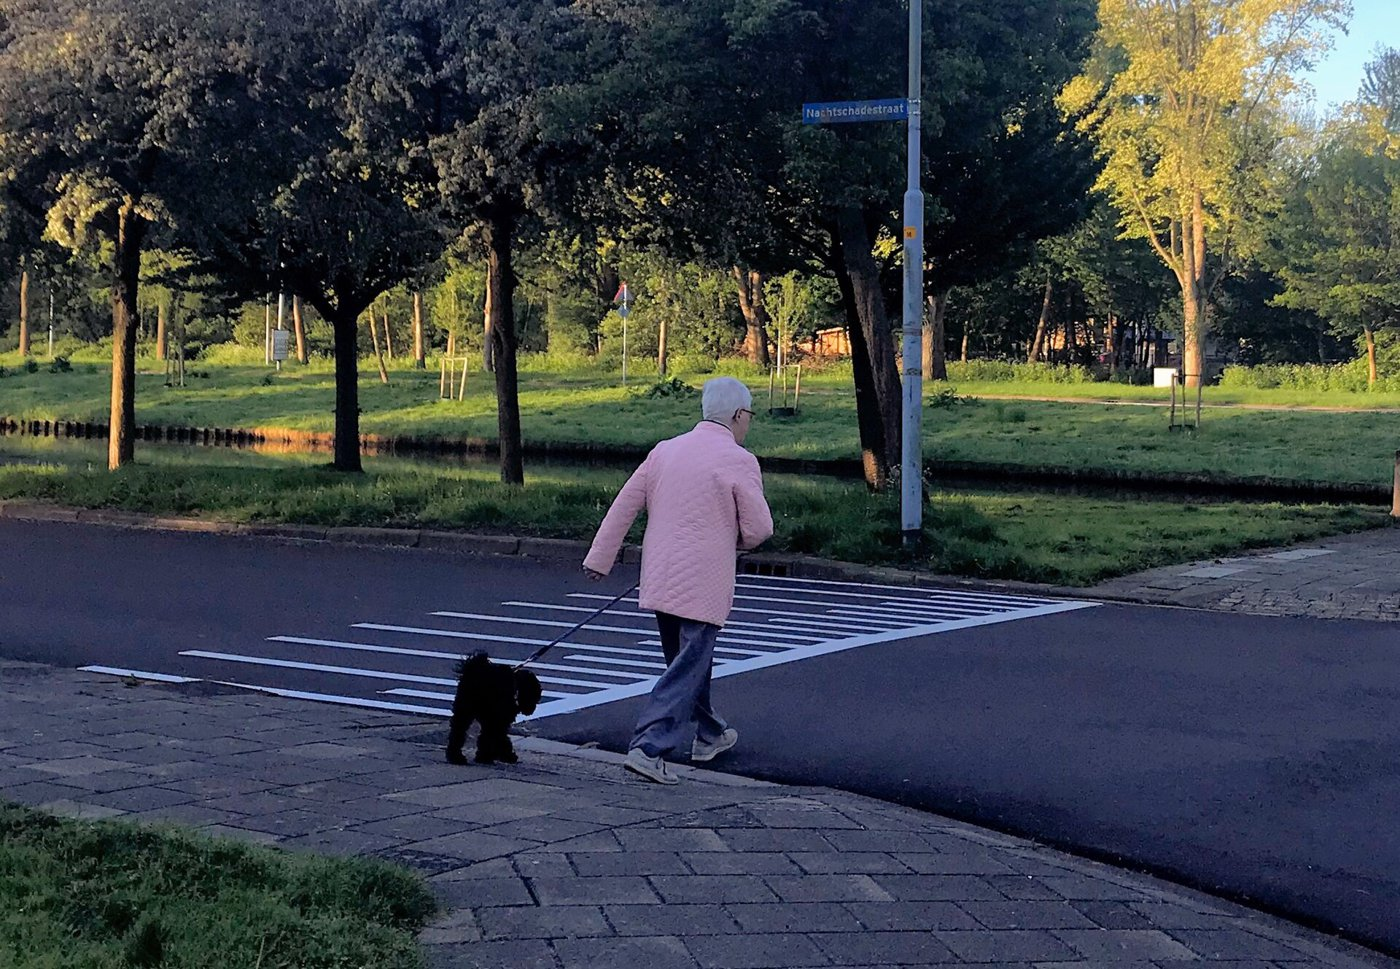
\includegraphics[height=0.40\textheight]{ch7_dog_walking_2018.jpg}\\[1mm]
\imgcap{O plimbare cu cîinele: două traiectorii care nu se îndepărtează mult una de alta}
\imgcredit{https://commons.wikimedia.org/wiki/File:Dog_walking_woman.jpg}{Foto: Amin (2018); CC BY-SA 4.0; Wikimedia Commons}
\end{column}
\begin{column}{0.58\textwidth}
\begin{itemize}
    \item \refMurray: o femeie beată iese din local și rătăcește: traiectoria ei $x_t$ este un mers aleator
    \begin{itemize}
        \item cîinele ei rătăcește și el: $y_t$ este tot un mers aleator
        \item distanța dintre doi trecători \textbf{independenți} crește fără limită, ca $\sqrt{t}$
    \end{itemize}
    \item Dar cîinele îi aude strigătul și aleargă înapoi; ea aude cîinele și se întoarce spre el
    \begin{itemize}
        \item fiecare corectează o parte din distanță: $\Delta x_t = c\,(y_{t-1} - x_{t-1}) + u_t$, $\Delta y_t = d\,(x_{t-1} - y_{t-1}) + w_t$
        \item ambele traiectorii rămîn imprevizibile, dar distanța $y_t - x_t$ rămîne mărginită: \textbf{cointegrare} cu \textbf{corecția erorii}
    \end{itemize}
\end{itemize}
\end{column}
\end{columns}
\end{frame}

\begin{frame}{Femeia beată și cîinele ei prin simulare}
\itemsize{\footnotesize}
\begin{center}
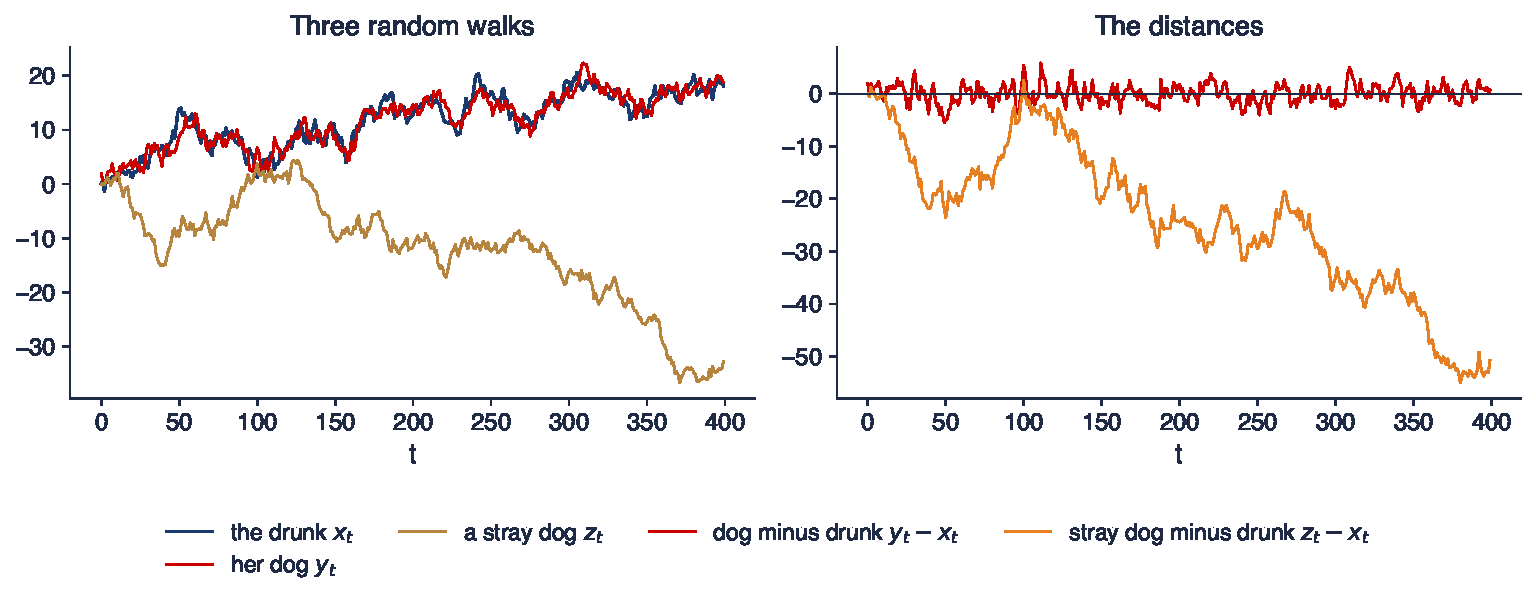
\includegraphics[width=0.97\textwidth,height=0.56\textheight,keepaspectratio]{tsa_ch7_drunk_dog.pdf}
\end{center}
\vspace{-0.25cm}
\begin{itemize}
    \item $T = 400$, șocuri gaussiene; $c = 0{,}15$, $d = 0{,}25$; un cîine fără stăpîn $z_t$ este un mers aleator independent, cu aceeași varianță a șocurilor
\end{itemize}
\quantlet{TSA\_ch7\_common\_trends}{\qlurl{TSA_ch7_common_trends}}
\end{frame}

\begin{frame}{Interpretarea simulării}
\itemsize{\small}
\begin{itemize}
    \item Fiecare traiectorie este $I(1)$: ADF pe $x_t$ dă p = 0{,}21
    \begin{itemize}
        \item distanța $y_t - x_t$ este un AR(1) cu $\rho = 1 - c - d = 0{,}6$: ADF p $<$\,0{,}001, abaterea standard 1{,}9
        \item distanța față de cîinele fără stăpîn rătăcește: ADF p = 0{,}81, abaterea standard 14{,}1
    \end{itemize}
    \item Jumătate dintr-o distanță dispare în $\ln 0{,}5/\ln 0{,}6 = 1{,}4$ pași: \textbf{timpul de înjumătățire} (secțiunea 3)
    \begin{itemize}
        \item știind unde este femeia, știm unde să căutăm cîinele, deși niciuna dintre traiectorii nu poate fi prognozată
    \end{itemize}
\end{itemize}
\end{frame}

\begin{frame}{Definiția cointegrării}
\itemsize{\small}
\begin{itemize}
    \item \textbf{Definiție} \refEG: componentele lui $\mathbf y_t = (y_{1t}, \dots, y_{nt})^\top$ sînt \textbf{cointegrate de ordinul (1,1)}, $\mathbf y_t \sim CI(1,1)$, dacă
    \begin{itemize}
        \item fiecare componentă este $I(1)$ (\tsachlink{https://danpele.github.io/Time-Series-Analysis/RO/Cursuri/capitol3_radacini_unitare_modele_arima.pdf}{Capitolul 3}: staționară după o diferențiere) și
        \item o anumită combinație liniară $\beta^\top \mathbf y_t$, cu $\beta \neq 0$, este $I(0)$: staționară
    \end{itemize}
    \item $\beta$ este \textbf{vectorul de cointegrare}; $u_t = \beta^\top \mathbf y_t - \mu$ este \textbf{eroarea de echilibru}
    \begin{itemize}
        \item $\beta$ este unic doar pînă la o constantă multiplicativă: și $2\beta$ este bun; \textbf{normalizăm} un coeficient la 1, de exemplu $\beta = (1, -b)^\top$
        \item cu $n$ variabile pot exista cel mult $r = n - 1$ vectori de cointegrare independenți; $r$ este \textbf{rangul de cointegrare}
    \end{itemize}
    \item Cointegrarea este o proprietate a \textbf{nivelurilor}: diferențierea datelor distruge informația din $\beta^\top \mathbf y_t$
\end{itemize}
\end{frame}

\begin{frame}{Trenduri stochastice comune}
\itemsize{\small}
\begin{itemize}
    \item Fie $x_t = x_{t-1} + \varepsilon_t$ (un mers aleator) și $y_t = b\,x_t + u_t$, cu $u_t$ staționar
    \begin{itemize}
        \item ambele serii conțin același trend stochastic $\sum_{s \le t} \varepsilon_s$; $y_t - b x_t = u_t$ îl elimină
    \end{itemize}
    \item Reprezentarea prin \textbf{trenduri comune} \refSW: $n$ variabile cu $r$ vectori de cointegrare sînt antrenate de $n - r$ trenduri stochastice comune
    \begin{itemize}
        \item $r = 0$: $n$ trenduri separate, fără cointegrare; $r = n - 1$: un singur trend, comun tuturor
        \item exemplu: trei randamente (la 1, 5 și 10 ani) cu $r = 2$ au un singur trend comun, \textbf{nivelul} ratelor dobînzii (secțiunea 5)
    \end{itemize}
    \item \textbf{Exemplu rezolvat}: $x_t$ mers aleator, $y_t = 2x_t + u_t$, $z_t = -x_t + v_t$ ($u_t$, $v_t$ staționare)
    \begin{itemize}
        \item $n = 3$, un singur trend comun, deci $r = 2$: de exemplu $\beta_1 = (1, -2, 0)^\top$ și $\beta_2 = (0, 1, 2)^\top$ (deoarece $y_t + 2z_t = u_t + 2v_t$)
    \end{itemize}
\end{itemize}
\end{frame}

\begin{frame}{Cointegrarea în teoria economică}
\itemsize{\small}
\begin{itemize}
    \item \textbf{Paritatea puterii de cumpărare}: $s_t = p_t - p^*_t + q_t$, cu cursul real $q_t$ staționar (secțiunea 8)
    \begin{itemize}
        \item $s_t$: logaritmul cursului (lei pentru un euro); $p_t$, $p^*_t$: logaritmii nivelurilor prețurilor în țară și în străinătate
    \end{itemize}
    \item \textbf{Structura la termen a ratelor dobînzii}: conform ipotezei așteptărilor, diferența (spread-ul) dintre un randament pe termen lung și unul pe termen scurt este staționară \refCS
    \item \textbf{Consum și venit}: „marele raport” $c_t - y_t$ (în logaritmi) este stabil dacă consumul urmează venitul permanent
    \item \textbf{Prețul spot și prețul futures}, un indice și un fond care îl replică: arbitrajul menține diferența mică
    \item \textbf{Acțiunile unor firme similare}: aceleași șocuri sectoriale; baza pairs trading (secțiunea 9)
\end{itemize}
\end{frame}

\begin{frame}{Patru perechi de serii cu trend}
\itemsize{\footnotesize}
\begin{center}
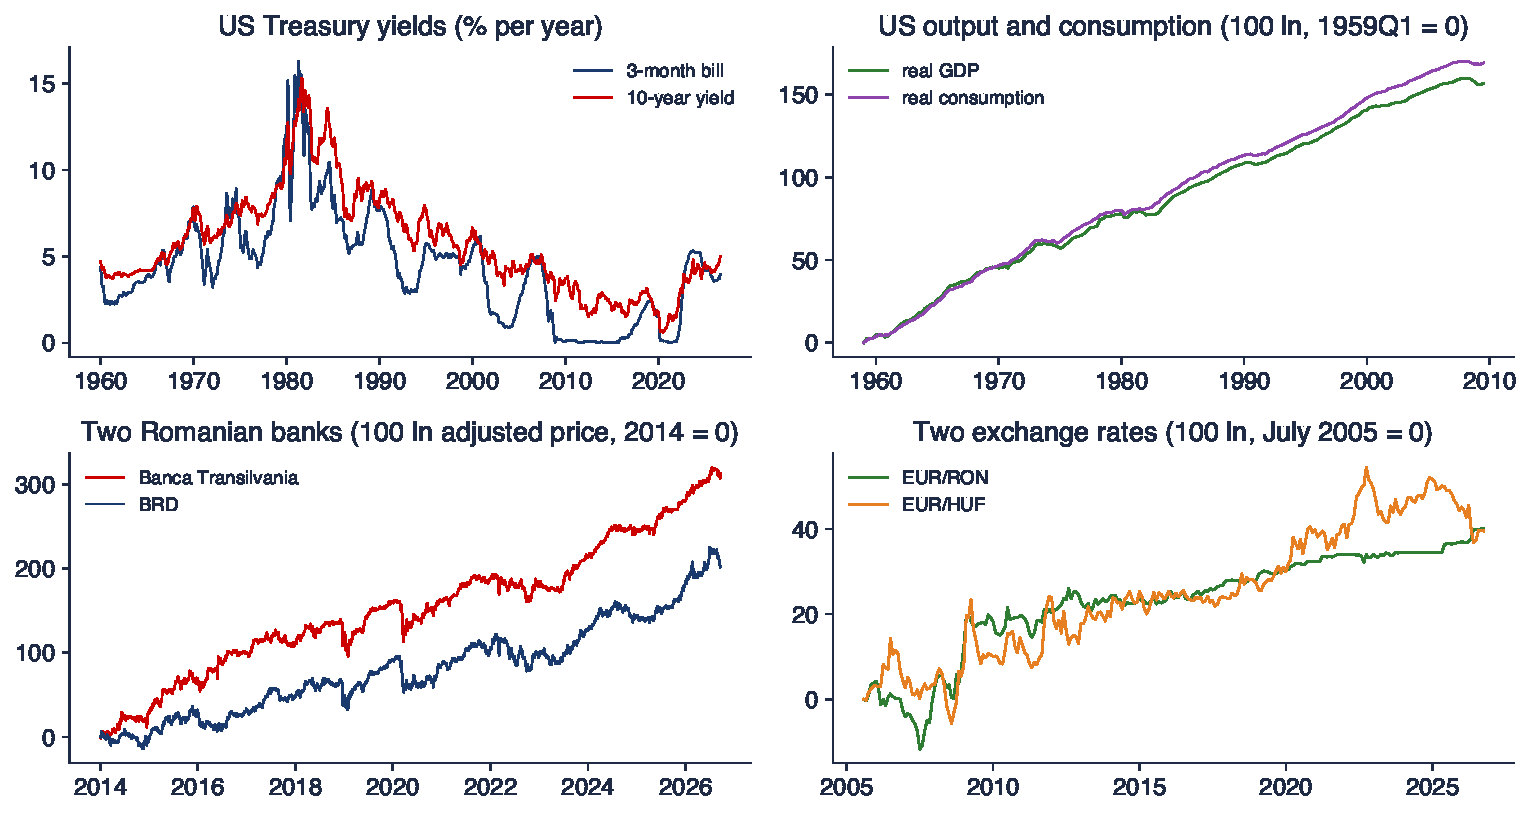
\includegraphics[width=0.97\textwidth,height=0.58\textheight,keepaspectratio]{tsa_ch7_examples.pdf}
\end{center}
\vspace{-0.25cm}
\begin{itemize}
    \item Randamentele titlurilor de stat americane (FRED, lunar, din 1960); PIB-ul și consumul real al SUA (macrodata din statsmodels, 1959--2009); Banca Transilvania și BRD (prețuri zilnice ajustate); EUR/RON și EUR/HUF (cursuri de referință BNR, la sfîrșitul lunii)
\end{itemize}
\quantlet{TSA\_ch7\_common\_trends}{\qlurl{TSA_ch7_common_trends}}
\end{frame}

\begin{frame}{Interpretarea celor patru perechi}
\itemsize{\small}
\begin{itemize}
    \item Fiecare serie este $I(1)$ (\tsachlink{https://danpele.github.io/Time-Series-Analysis/RO/Cursuri/capitol3_radacini_unitare_modele_arima.pdf}{Capitolul 3}); întrebarea este dacă cele două serii ale unei perechi evoluează \textbf{împreună} pe termen lung
    \begin{itemize}
        \item testul Engle--Granger (secțiunea 2), valoarea critică de 5\% circa $-3{,}34$
    \end{itemize}
    \item Randamentele: $\tau = -3{,}35$, p = 0{,}048: la limită; consumul și venitul: $\tau = -3{,}54$, p = 0{,}029
    \item Cele două bănci: $\tau = -4{,}33$, p = 0{,}002: cointegrate în acest eșantion
    \item EUR/RON și EUR/HUF: $\tau = -2{,}47$, p = 0{,}294: \textbf{nu} sînt cointegrate
    \begin{itemize}
        \item deși au crescut cu valori apropiate, iar $R^2 = 0{,}79$ în niveluri: o direcție comună nu este un trend comun
    \end{itemize}
\end{itemize}
\end{frame}

\begin{frame}{Întrebare pentru sală}
\itemsize{\small}
\begin{itemize}
    \item \textbf{Întrebare}: două serii $I(1)$ au în niveluri o corelație de 0,95. Sînt ele cointegrate?
    \begin{itemize}
        \item \textbf{Răspuns}: nu putem spune: mersurile aleatoare fără legătură au adesea corelații mari (\tsachlink{https://danpele.github.io/Time-Series-Analysis/RO/Cursuri/capitol3_radacini_unitare_modele_arima.pdf}{Capitolul 3}); doar un test pe eroarea de echilibru decide
    \end{itemize}
    \item \textbf{Întrebare}: două serii cointegrate au o corelație de 0,2 între variațiile lor zilnice. Este o contradicție?
    \begin{itemize}
        \item \textbf{Răspuns}: nu: cointegrarea privește termenul lung; pe termen scurt variațiile pot fi aproape necorelate
    \end{itemize}
\end{itemize}
\end{frame}

\begin{frame}{Recapitulare: ideea de cointegrare}
\itemsize{\small}
\begin{itemize}
    \item Seriile $I(1)$ sînt cointegrate dacă o combinație $\beta^\top \mathbf y_t$ este staționară: un echilibru pe termen lung
    \item Echivalent, au trenduri stochastice comune: $n$ variabile, $r$ vectori, $n - r$ trenduri
    \item Teoria sugerează cointegrarea (condiții de paritate, spread-uri, rapoarte mari), dar datele trebuie să o confirme
\end{itemize}
\end{frame}


%=============================================================================
\section{Metoda Engle--Granger în doi pași}
%=============================================================================

\begin{frame}{Doi pași}
\itemsize{\small}
\begin{itemize}
    \item \textbf{Pasul 1}: estimăm relația pe termen lung prin OLS (ordinary least squares, metoda celor mai mici pătrate) în niveluri: $y_t = a + b\,x_t + u_t$
    \begin{itemize}
        \item păstrăm reziduurile $\hat u_t = y_t - \hat a - \hat b x_t$
        \item dacă seriile sînt cointegrate, $\hat b$ este \textbf{superconsistent}: eroarea lui scade ca $1/T$, mai repede decît de obicei ($1/\sqrt{T}$)
    \end{itemize}
    \item \textbf{Pasul 2}: un test ADF (\tsachlink{https://danpele.github.io/Time-Series-Analysis/RO/Cursuri/capitol3_radacini_unitare_modele_arima.pdf}{Capitolul 3}) pe reziduuri, fără constantă: $\Delta\hat u_t = \gamma\,\hat u_{t-1} + \sum_{j=1}^{k}\delta_j\Delta\hat u_{t-j} + e_t$
    \begin{itemize}
        \item $H_0$: $\gamma = 0$, reziduurile au o rădăcină unitară: \textbf{fără cointegrare}; $H_1$: $\gamma < 0$: cointegrare
        \item statistica $\tau = \hat\gamma/\mathrm{SE}(\hat\gamma)$; respingem $H_0$ cînd $\tau$ este sub valoarea critică
    \end{itemize}
    \item Testare prealabilă: fiecare serie trebuie să fie $I(1)$; o serie $I(0)$ și una $I(1)$ nu pot fi cointegrate
\end{itemize}
\end{frame}

\begin{frame}{Motivul pentru care tabelul Dickey--Fuller este greșit aici}
\itemsize{\small}
\begin{itemize}
    \item OLS alege $\hat b$ astfel încît varianța reziduurilor să fie cît mai mică
    \begin{itemize}
        \item deci $\hat u_t$ pare mai staționar decît adevăratul $u_t$, chiar și atunci cînd nu există cointegrare
        \item în ipoteza $H_0$, statistica $\tau$ este deplasată la stînga distribuției Dickey--Fuller
    \end{itemize}
    \item Valorile critice depind de numărul de variabile $n$ și de termenii determiniști din pasul 1
    \begin{itemize}
        \item tabele: \refEG\ (prin simulare), apoi \refMacKinnon\ și \refMacKinnonb, folosite de \texttt{statsmodels} (\texttt{coint})
    \end{itemize}
    \item Cu $\beta$ \textbf{cunoscut} din teorie (de exemplu un spread, $\beta = (1, -1)^\top$), nu se estimează nimic: se aplică testul ADF obișnuit, cu tabelul lui
\end{itemize}
\end{frame}

\begin{frame}{Distribuția în ipoteza nulă prin simulare}
\itemsize{\footnotesize}
\begin{center}
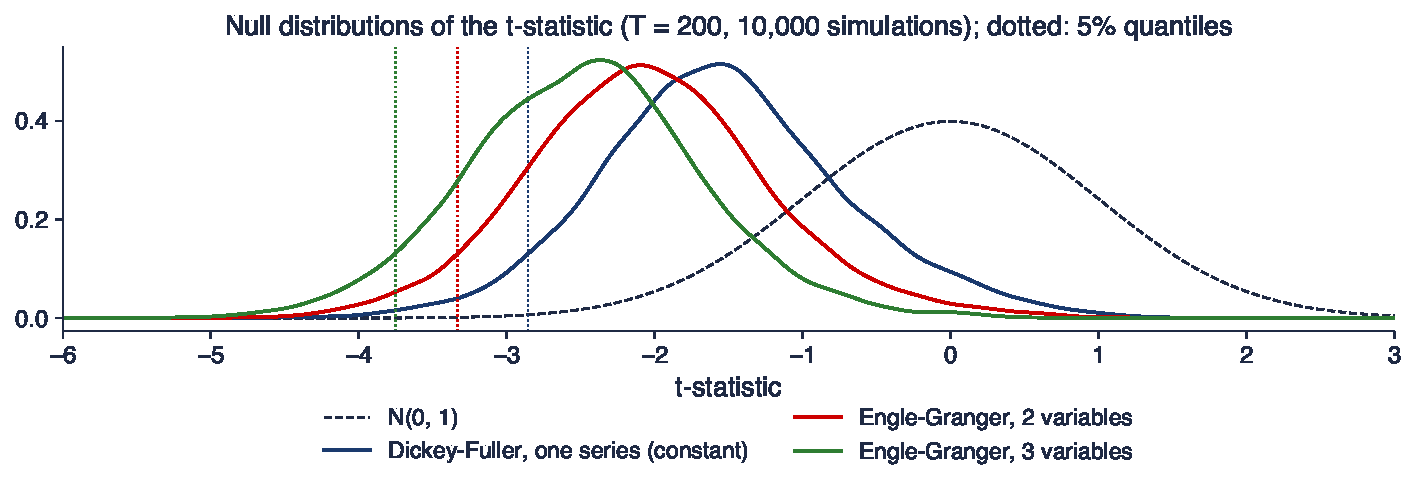
\includegraphics[width=0.97\textwidth,height=0.55\textheight,keepaspectratio]{tsa_ch7_eg_dist.pdf}
\end{center}
\vspace{-0.25cm}
\begin{itemize}
    \item 10\,000 de eșantioane de $T = 200$ mersuri aleatoare gaussiene independente; pasul 1 cu constantă, pasul 2 fără decalaje
\end{itemize}
\quantlet{TSA\_ch7\_engle\_granger}{\qlurl{TSA_ch7_engle_granger}}
\end{frame}

\begin{frame}{Interpretarea simulării}
\itemsize{\small}
\begin{itemize}
    \item Cuantilele de 5\%: $-2{,}86$ (o serie, Dickey--Fuller), $-3{,}33$ (2 variabile), $-3{,}75$ (3 variabile)
    \begin{itemize}
        \item valorile MacKinnon pentru $T = 200$: $-2{,}88$; $-3{,}37$; $-3{,}78$: simularea le reproduce
    \end{itemize}
    \item Folosind valoarea Dickey--Fuller $-2{,}88$ pentru reziduuri, am respinge o ipoteză $H_0$ adevărată în 14{,}5\% din eșantioane cu 2 variabile și în 30{,}3\% cu 3
    \begin{itemize}
        \item în loc de 5\%: am „găsi” cointegrare mult prea des
    \end{itemize}
    \item Mai multe variabile îi dau metodei OLS mai multă libertate de ajustare, de unde valori critice mai negative
\end{itemize}
\end{frame}

\begin{frame}{Valorile critice ale testului Engle--Granger}
\itemsize{\small}
\begin{center}
\footnotesize
\begin{tabular}{lcccccc}
\toprule
\textbf{Variabile $n$} & \multicolumn{3}{c}{\textbf{constantă}} & \multicolumn{3}{c}{\textbf{constantă și trend}} \\
 & 1\% & 5\% & 10\% & 1\% & 5\% & 10\% \\
\midrule
1 (Dickey--Fuller) & $-3{,}43$ & $-2{,}86$ & $-2{,}57$ & $-3{,}96$ & $-3{,}41$ & $-3{,}13$ \\
2 & $-3{,}90$ & $-3{,}34$ & $-3{,}04$ & $-4{,}33$ & $-3{,}78$ & $-3{,}50$ \\
3 & $-4{,}29$ & $-3{,}74$ & $-3{,}45$ & $-4{,}66$ & $-4{,}12$ & $-3{,}84$ \\
4 & $-4{,}64$ & $-4{,}10$ & $-3{,}81$ & $-4{,}97$ & $-4{,}43$ & $-4{,}15$ \\
\bottomrule
\end{tabular}
\end{center}
\begin{itemize}
    \item Valori asimptotice ($T \to \infty$) din \refMacKinnonb; pentru $T$ finit, valorile sînt puțin mai negative
    \item Citiți rîndul cu numărul \textbf{total} de variabile din regresie, inclusiv $y_t$
    \item Constantă și trend în pasul 1: cînd seriile au derive pe care relația nu le anulează
\end{itemize}
\end{frame}

\begin{frame}{Testul Phillips--Ouliaris}
\itemsize{\small}
\begin{itemize}
    \item \refPO: același pas 1 și aceeași ipoteză $H_0$ (fără cointegrare)
    \begin{itemize}
        \item pasul 2: o regresie Dickey--Fuller \textbf{fără} diferențe decalate; statistica $t$ este corectată cu varianța pe termen lung a reziduurilor (ca în testul Phillips--Perron din \tsachlink{https://danpele.github.io/Time-Series-Analysis/RO/Cursuri/capitol3_radacini_unitare_modele_arima.pdf}{Capitolul 3})
        \item două versiuni: $Z_t$ (raportul $t$ corectat) și $Z_\alpha$ ($T\hat\gamma$ corectat); valorile critice ale lui $Z_t$ sînt cele Engle--Granger
    \end{itemize}
    \item De ce două teste?
    \begin{itemize}
        \item Engle--Granger depinde de numărul de decalaje $k$ ales după AIC; Phillips--Ouliaris depinde de lățimea de bandă a varianței pe termen lung
        \item cînd concordă, verdictul este robust; cînd nu concordă, examinăm graficul reziduurilor și eșantionul
    \end{itemize}
    \item În Python: \texttt{coint(y, x)} din \texttt{statsmodels}; \texttt{phillips\_ouliaris(y, x, test\_type="Zt")} din \texttt{arch}
\end{itemize}
\end{frame}

\begin{frame}{Exemplu rezolvat: consumul și venitul în SUA}
\itemsize{\small}
\begin{itemize}
    \item Datele: $c_t$, $y_t$ = 100 $\times$ logaritmul consumului real și al PIB-ului real, trimestrial, T1 1959--T3 2009 (203 de trimestre)
    \begin{itemize}
        \item testare prealabilă: ADF cu trend, p = 0{,}31 pentru $c_t$ și 0{,}39 pentru $y_t$: ambele $I(1)$
    \end{itemize}
    \item Pasul 1: $\hat c_t = -107{,}6 + 1{,}075\,y_t$, $R^2 = 0{,}9992$, DW $= 0{,}24$
    \begin{itemize}
        \item panta este apropiată de 1: o pondere stabilă a consumului; dar $R^2$ și DW singure nu dovedesc nimic
    \end{itemize}
    \item Pasul 2: $\tau = -3{,}54$ cu 0 decalaje; valoarea critică de 5\% pentru $n = 2$, $T = 203$: $-3{,}37$
    \begin{itemize}
        \item $-3{,}54 < -3{,}37$: respingem „fără cointegrare” la 5\% (p = 0{,}029); Phillips--Ouliaris: $Z_t = -3{,}52$, p = 0{,}031
        \item cu valoarea Dickey--Fuller ($-2{,}88$) decizia ar fi aceeași aici, dar din motive greșite
    \end{itemize}
\end{itemize}
\end{frame}

\begin{frame}{Reziduurile din pasul 1}
\itemsize{\footnotesize}
\begin{center}
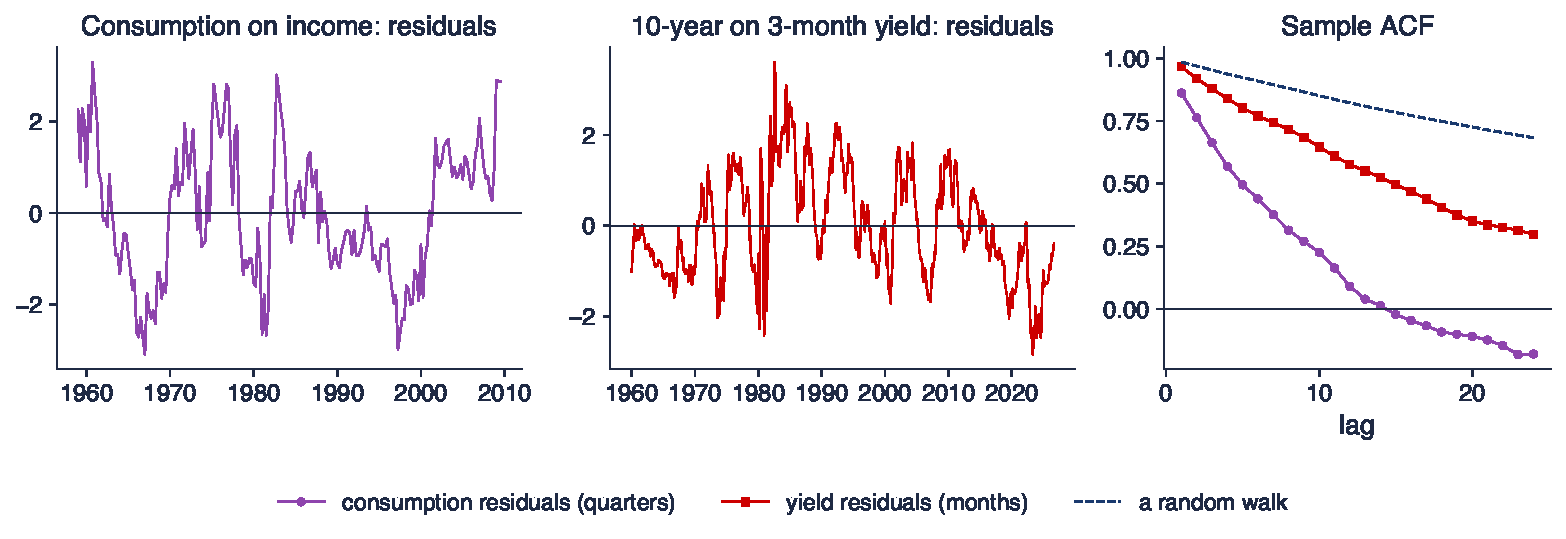
\includegraphics[width=0.97\textwidth,height=0.54\textheight,keepaspectratio]{tsa_ch7_eg_steps.pdf}
\end{center}
\vspace{-0.25cm}
\begin{itemize}
    \item Stînga și centru: $\hat u_t$ pentru consumul pe venit și pentru randamentul la 10 ani pe cel la 3 luni; dreapta: ACF de selecție a lor și a unui mers aleator simulat
\end{itemize}
\quantlet{TSA\_ch7\_engle\_granger}{\qlurl{TSA_ch7_engle_granger}}
\end{frame}

\begin{frame}{Interpretarea reziduurilor}
\itemsize{\small}
\begin{itemize}
    \item Consumul: $\hat\rho(1) = 0{,}86$, dar $\hat\rho(8) = 0{,}31$: abateri de 1--3\% care se reduc mult în aproximativ doi ani
    \item Randamentele: $\hat\rho(1) = 0{,}97$, $\hat\rho(12) = 0{,}58$: abateri foarte persistente; un test la limită ($\tau = -3{,}35$, p = 0{,}048)
    \begin{itemize}
        \item persistența ridicată este situația obișnuită: puterea testului împotriva unui $\rho$ apropiat de 1 este mică (\tsachlink{https://danpele.github.io/Time-Series-Analysis/RO/Cursuri/capitol3_radacini_unitare_modele_arima.pdf}{Capitolul 3})
    \end{itemize}
    \item Un mers aleator descrește mult mai lent: ACF singură nu poate tranșa întrebarea; testul poate
\end{itemize}
\end{frame}

\begin{frame}{Engle--Granger și Phillips--Ouliaris pe date reale}
\itemsize{\small}
\begin{center}
\scriptsize
\begin{tabular}{llrrrrrr}
\toprule
\textbf{Regresia} & \textbf{Frecv.} & $T$ & $\hat b$ & $\tau$ (k) & p & $Z_t$ & p \\
\midrule
SUA: consumul pe venit & trimestrial & 203 & 1{,}07 & $-3{,}54$ (0) & 0{,}029 & $-3{,}52$ & 0{,}031 \\
SUA: 10 ani pe 3 luni & lunar & 801 & 0{,}86 & $-3{,}35$ (20) & 0{,}048 & $-4{,}04$ & 0{,}006 \\
TLV pe BRD (din 2014) & zilnic & 3\,176 & 1{,}36 & $-4{,}33$ (3) & 0{,}002 & $-4{,}14$ & 0{,}005 \\
BRD pe TLV (din 2014) & zilnic & 3\,176 & 0{,}71 & $-4{,}16$ (3) & 0{,}004 & $-4{,}02$ & 0{,}007 \\
TLV pe BRD (din 2010) & zilnic & 4\,187 & 1{,}68 & $-1{,}82$ (3) & 0{,}622 & $-1{,}83$ & 0{,}619 \\
EUR/RON pe EUR/HUF & lunar & 255 & 0{,}71 & $-2{,}47$ (0) & 0{,}294 & $-2{,}43$ & 0{,}309 \\
România: consumul pe PIB & trimestrial & 126 & 1{,}46 & $-2{,}32$ (8) & 0{,}363 & $-6{,}80$ & $<$\,0{,}001 \\
\bottomrule
\end{tabular}
\end{center}
\begin{itemize}
    \item $\tau$: statistica Engle--Granger ($k$ decalaje după AIC); valori p din \refMacKinnonb\ pentru 2 variabile; $Z_t$: Phillips--Ouliaris
    \item Băncile: prețuri ajustate din data/market; România: consumul gospodăriilor și PIB-ul, Eurostat, volume înlănțuite, ajustate sezonier, din 1995
\end{itemize}
\end{frame}

\begin{frame}{Interpretarea tabelului}
\itemsize{\small}
\begin{itemize}
    \item \textbf{Normalizarea}: TLV pe BRD și BRD pe TLV dau valori $\tau$ diferite ($-4{,}33$ și $-4{,}16$) și pante care nu sînt exact inverse una alteia
    \begin{itemize}
        \item Engle--Granger depinde de variabila aleasă în stînga; aici verdictul este același
    \end{itemize}
    \item \textbf{Eșantionul}: din 2010 aceleași bănci nu sînt cointegrate (p = 0{,}622); din 2014 sînt (p = 0{,}002)
    \begin{itemize}
        \item alegerea datei de început după examinarea datelor este o formă de data snooping (căutare în date pînă la găsirea unui rezultat)
    \end{itemize}
    \item \textbf{Cele două teste nu concordă} pentru România: Engle--Granger p = 0{,}363 cu 8 decalaje, Phillips--Ouliaris p $<$\,0{,}001
    \begin{itemize}
        \item panta 1{,}46 este departe de 1: ponderea consumului a crescut puternic; Seminarul 7 (B2) discută acest caz
    \end{itemize}
\end{itemize}
\end{frame}

\begin{frame}{Limitele metodei Engle--Granger}
\itemsize{\small}
\begin{itemize}
    \item \textbf{Cel mult un} vector de cointegrare: cu $n \ge 3$ variabile pot exista mai mulți (secțiunile 4--5)
    \item \textbf{Normalizarea}: rezultatele depind de variabila pusă în stînga
    \item \textbf{Inferența asupra lui $\hat b$}: superconsistent, dar deplasat în eșantioane mici, iar statisticile $t$ din OLS \textbf{nu} sînt valide
    \begin{itemize}
        \item remediu: OLS dinamic (DOLS) \refSWd, cu valori anticipate și decalate ale lui $\Delta x_t$, dă erori standard valide
    \end{itemize}
    \item \textbf{Erori în doi pași}: greșelile din pasul 1 se transmit în pasul 2; puterea este mică împotriva unei ajustări lente
    \begin{itemize}
        \item metoda Johansen (secțiunea 5) estimează totul deodată, prin verosimilitate maximă
    \end{itemize}
\end{itemize}
\end{frame}

\begin{frame}{Studiu de caz: Engle și Granger (1987)}
\itemsize{\small}
\begin{columns}[T]
\begin{column}{0.30\textwidth}
\centering
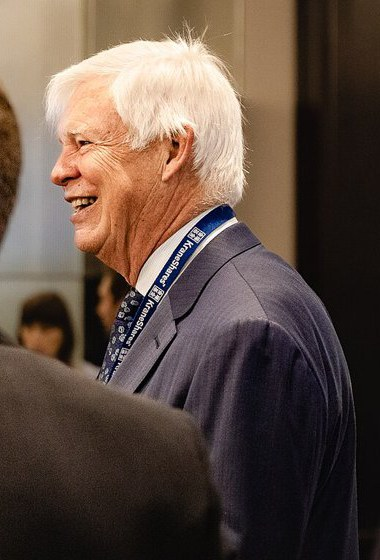
\includegraphics[height=0.44\textheight]{ch7_robert_engle_2022.jpg}\\[1mm]
\imgcap{Robert Engle (2022); Premiul Nobel pentru economie 2003}
\imgcredit{https://commons.wikimedia.org/wiki/File:0603_KRBN-RobertEngle-JonDemske-10.jpg}{Foto: Jon Demske (2022); CC BY-SA 4.0; Wikimedia Commons}
\end{column}
\begin{column}{0.66\textwidth}
\begin{itemize}
    \item \textbf{Întrebarea}: cum modelăm serii $I(1)$ legate pe termen lung, fără regresii false și fără a elimina prin diferențiere informația pe termen lung?
    \begin{itemize}
        \item \refEG, scrisă la Universitatea California din San Diego, una dintre cele mai citate lucrări din econometrie
    \end{itemize}
    \item \textbf{Contribuția}
    \begin{itemize}
        \item definiția cointegrării și teorema de reprezentare (secțiunea 4): cointegrare $\Leftrightarrow$ corecția erorii
        \item estimatorul în doi pași și testele pe reziduuri, cu valori critice obținute prin simulare
        \item aplicații pe serii din SUA, precum consumul și venitul, prețurile și salariile, ratele dobînzii pe termen scurt și lung
    \end{itemize}
    \item \textbf{Recunoaștere}: Premiul Nobel 2003, Granger pentru cointegrare, Engle pentru ARCH (\tsachlink{https://danpele.github.io/Time-Series-Analysis/RO/Cursuri/capitol5_volatilitate_conditionata_garch.pdf}{Capitolul 5})
\end{itemize}
\end{column}
\end{columns}
\end{frame}

\begin{frame}{Recapitulare: metoda Engle--Granger}
\itemsize{\small}
\begin{itemize}
    \item Pasul 1: OLS în niveluri ($\hat b$ superconsistent); pasul 2: ADF pe reziduuri, $H_0$: fără cointegrare
    \item Valorile critice Engle--Granger (MacKinnon), mai negative decît cele Dickey--Fuller și dependente de $n$
    \item Verificăm cu Phillips--Ouliaris, cu normalizarea inversă și cu un alt eșantion
\end{itemize}
\end{frame}


%=============================================================================
\section{Modele cu corecția erorii}
%=============================================================================

\begin{frame}{Modelul cu corecția erorii}
\itemsize{\small}
\begin{itemize}
    \item Cu $u_{t-1} = y_{t-1} - a - b x_{t-1}$ (eroarea de echilibru din perioada anterioară), \textbf{modelul cu corecția erorii} (ECM) este
    \begin{itemize}
        \item $\Delta y_t = c + \gamma\,u_{t-1} + \delta_0\,\Delta x_t + \sum_{j \ge 1}(\phi_j\Delta y_{t-j} + \delta_j\Delta x_{t-j}) + \varepsilon_t$
    \end{itemize}
    \item Toți termenii sînt staționari: OLS și testele $t$ obișnuite sînt valide (cu $\hat u_{t-1}$ din pasul 1)
    \begin{itemize}
        \item $b$: efectul \textbf{pe termen lung} al lui $x$ asupra lui $y$; $\delta_0$: efectul \textbf{pe termen scurt} (în aceeași perioadă)
        \item $\gamma$: \textbf{viteza de ajustare}; corecția erorii cere $-2 < \gamma < 0$
    \end{itemize}
    \item Interpretare: dacă $y_{t-1}$ a fost peste echilibru ($u_{t-1} > 0$) și $\gamma < 0$, atunci $y_t$ tinde să scadă: o fracțiune $|\gamma|$ din distanță se închide în fiecare perioadă
\end{itemize}
\end{frame}

\begin{frame}{Viteza de ajustare și timpul de înjumătățire}
\itemsize{\small}
\begin{itemize}
    \item Fără șocuri noi, eroarea de echilibru evoluează după $u_t = (1 + \gamma)\,u_{t-1}$, deci $u_h = (1 + \gamma)^h u_0$
    \begin{itemize}
        \item (într-un sistem cu două variabile în care se ajustează doar $y$)
    \end{itemize}
    \item \textbf{Timpul de înjumătățire}: numărul de perioade după care a dispărut jumătate dintr-o abatere
    \begin{itemize}
        \item $(1 + \gamma)^{h} = 0{,}5 \;\Rightarrow\; h_{1/2} = \ln 0{,}5 / \ln(1 + \gamma)$
    \end{itemize}
    \item \textbf{Exemplu rezolvat}: $\gamma = -0{,}2$, $h_{1/2} = \ln 0{,}5/\ln 0{,}8 = 3{,}1$ perioade
    \begin{itemize}
        \item în luni: circa trei luni pentru jumătate dintr-o abatere; în trimestre: trei trimestre
    \end{itemize}
    \item Comparăm timpii de înjumătățire doar în aceeași unitate de timp: un $\gamma$ lunar și unul trimestrial nu sînt comparabile
\end{itemize}
\end{frame}

\begin{frame}{Timpi de înjumătățire: teorie și estimări}
\itemsize{\footnotesize}
\begin{center}
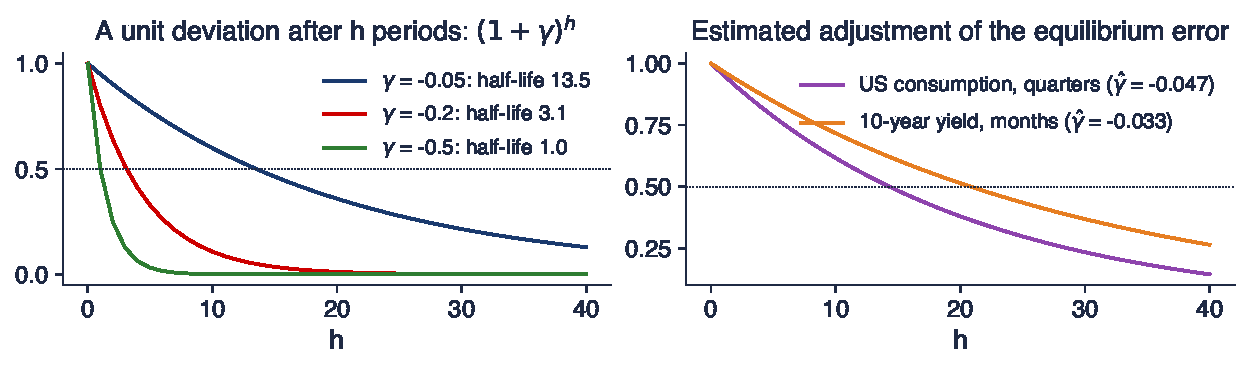
\includegraphics[width=0.97\textwidth,height=0.55\textheight,keepaspectratio]{tsa_ch7_ecm.pdf}
\end{center}
\vspace{-0.25cm}
\begin{itemize}
    \item Stînga: $(1 + \gamma)^h$ pentru trei viteze; dreapta: descreșterea implicată de modelele ECM estimate pentru consumul din SUA (trimestre) și pentru randamentul la 10 ani (luni)
\end{itemize}
\quantlet{TSA\_ch7\_error\_correction}{\qlurl{TSA_ch7_error_correction}}
\end{frame}

\begin{frame}{Interpretarea modelelor ECM estimate}
\itemsize{\small}
\begin{itemize}
    \item Consumul: $\hat\gamma = -0{,}047$ ($t = -1{,}75$), timp de înjumătățire 14{,}3 trimestre; $\hat\delta_0 = 0{,}54$
    \begin{itemize}
        \item jumătate dintr-o creștere a venitului ajunge în consum în același trimestru; restul vine lent, iar termenul de ajustare este doar marginal semnificativ
    \end{itemize}
    \item Randamentul la 10 ani: $\hat\gamma = -0{,}033$ ($t = -4{,}94$), timp de înjumătățire 20{,}8 luni; $\hat\delta_0 = 0{,}38$
    \begin{itemize}
        \item și rata la 3 luni reacționează la aceeași distanță: $\hat\gamma = 0{,}024$ ($t = 2{,}08$), cu semn opus: ambele rate se apropie una de alta
    \end{itemize}
    \item Cînd ambele variabile se ajustează, un ECM cu o singură ecuație spune doar jumătate din poveste: de aici VECM (secțiunea 4)
\end{itemize}
\end{frame}

\begin{frame}{Exemplu rezolvat: un trimestru de consum}
\itemsize{\small}
\begin{itemize}
    \item ECM estimat (termenii principali): $\Delta c_t = 0{,}418 + 0{,}54\,\Delta y_t -0{,}047\,\hat u_{t-1} + \dots$, cu $\hat u_{t-1} = c_{t-1} - 1{,}075\,y_{t-1} - \hat a$
    \item Scenariu: consumul este cu $2\%$ peste echilibru ($\hat u_{t-1} = 2$), iar venitul crește cu $1\%$ în acest trimestru
    \begin{itemize}
        \item efectul pe termen scurt: $0{,}54 \times 1 = 0{,}537$; corecția erorii: $-0{,}047 \times 2 = -0{,}095$
        \item creșterea prognozată a consumului: circa $0{,}86\%$ (diferențele decalate sînt egale cu 0)
    \end{itemize}
    \item Fără termenul de corecție a erorii, modelul ar ignora faptul că deja consumul este prea mare
\end{itemize}
\end{frame}

\begin{frame}{Studiu de caz: funcția de consum DHSY (1978)}
\itemsize{\small}
\begin{itemize}
    \item \textbf{Întrebarea}: de ce prognozau atît de prost cheltuielile de consum din Marea Britanie funcțiile de consum din anii 1970, estimate în niveluri sau în diferențe?
    \begin{itemize}
        \item \refDHSY\ (Davidson, Hendry, Srba și Yeo, „DHSY”): date trimestriale pentru Marea Britanie, cheltuieli și venit
    \end{itemize}
    \item \textbf{Metoda}: un model în diferențe plus raportul logaritmic decalat dintre cheltuieli și venit, termenul de corecție a erorii
    \begin{itemize}
        \item o căutare de la general la particular, pornind de la un model dinamic amplu
    \end{itemize}
    \item \textbf{Moștenirea}: forma ECM a apărut prima; \refGranger\ și \refEG\ au arătat apoi de ce funcționează: cele două serii sînt cointegrate
    \begin{itemize}
        \item un test de cointegrare poate folosi și statistica $t$ a lui $\gamma$ din ECM, cu valori critice proprii \refBDM
    \end{itemize}
\end{itemize}
\end{frame}

\begin{frame}{Recapitulare: modele cu corecția erorii}
\itemsize{\small}
\begin{itemize}
    \item ECM: $\Delta y_t$ pe $\Delta x_t$, diferențe decalate și $\hat u_{t-1}$; toți termenii sînt staționari
    \item $\gamma < 0$: viteza de ajustare; timpul de înjumătățire $\ln 0{,}5/\ln(1 + \gamma)$, în unitățile datelor
    \item Termenul scurt ($\delta_0$) și termenul lung ($b$) într-o singură ecuație; dacă se ajustează mai multe variabile, avem nevoie de un sistem
\end{itemize}
\end{frame}


%=============================================================================
\section{Modelul VECM și teorema de reprezentare a lui Granger}
%=============================================================================

\begin{frame}{De la VAR la VECM}
\itemsize{\small}
\begin{itemize}
    \item \tsachlink{https://danpele.github.io/Time-Series-Analysis/RO/Cursuri/capitol6_modele_var_cauzalitate_granger.pdf}{Capitolul 6}: un VAR($p$) în niveluri, $\mathbf y_t = \mathbf c + A_1\mathbf y_{t-1} + \dots + A_p\mathbf y_{t-p} + \mathbf u_t$
    \begin{itemize}
        \item scădem $\mathbf y_{t-1}$ și regrupăm decalajele: același model sub forma \textbf{vectorială cu corecția erorii} (VECM)
    \end{itemize}
    \item $\Delta\mathbf y_t = \mathbf c + \Pi\,\mathbf y_{t-1} + \sum_{i=1}^{p-1}\Gamma_i\,\Delta\mathbf y_{t-i} + \mathbf u_t$, \quad $\Pi = A_1 + \dots + A_p - I$, \quad $\Gamma_i = -(A_{i+1} + \dots + A_p)$
    \item \textbf{Deducere} pentru $p = 2$: $\mathbf y_t - \mathbf y_{t-1} = (A_1 - I)\mathbf y_{t-1} + A_2\mathbf y_{t-2} + \mathbf u_t$; adunăm și scădem $A_2\mathbf y_{t-1}$:
    \begin{itemize}
        \item $\Delta\mathbf y_t = (A_1 + A_2 - I)\,\mathbf y_{t-1} - A_2\,\Delta\mathbf y_{t-1} + \mathbf u_t$: $\Pi = A_1 + A_2 - I$, $\Gamma_1 = -A_2$
    \end{itemize}
    \item VECM este o rescriere, nu un model nou: toată informația despre termenul lung se află în matricea $\Pi$
\end{itemize}
\end{frame}

\begin{frame}{Rangul matricei $\Pi$}
\itemsize{\small}
\begin{itemize}
    \item $\Delta\mathbf y_t$ este staționar; deci și $\Pi\mathbf y_{t-1}$ trebuie să fie staționar. Trei cazuri, după $r = \mathrm{rang}(\Pi)$:
    \item $r = 0$: $\Pi = 0$; fără cointegrare; modelul potrivit este un \textbf{VAR în diferențe}
    \item $r = n$: $\Pi$ are rang maxim; $\mathbf y_t$ este deja staționar; un \textbf{VAR în niveluri} (\tsachlink{https://danpele.github.io/Time-Series-Analysis/RO/Cursuri/capitol6_modele_var_cauzalitate_granger.pdf}{Capitolul 6})
    \item $0 < r < n$: \textbf{cointegrare} cu $r$ vectori; $\Pi = \alpha\beta^\top$, cu $\alpha$, $\beta$ de dimensiune $n \times r$
    \begin{itemize}
        \item $\beta^\top\mathbf y_{t-1}$: cele $r$ erori de echilibru; $\alpha$: \textbf{coeficienții de ajustare} (loadings), cît de puternic reacționează fiecare variabilă la fiecare eroare
        \item doar produsul este unic: $\alpha\beta^\top = (\alpha Q)(\beta Q^{-\top})^\top$ pentru orice $Q$ inversabilă; normalizăm $\beta$
    \end{itemize}
    \item Testarea cointegrării = testarea rangului lui $\Pi$ (secțiunea 5)
\end{itemize}
\end{frame}

\begin{frame}{Teorema de reprezentare a lui Granger}
\itemsize{\small}
\begin{itemize}
    \item \textbf{Teorema} \refEG: dacă $\mathbf y_t$ este $I(1)$ și cointegrat cu rangul $r$, atunci are o reprezentare VECM cu $\Pi = \alpha\beta^\top$, și reciproc
    \begin{itemize}
        \item cointegrare $\Leftrightarrow$ corecția erorii: eroarea de echilibru trebuie să influențeze variațiile
    \end{itemize}
    \item \textbf{Consecințe}
    \begin{itemize}
        \item un VAR în diferențe omite $\alpha\beta^\top\mathbf y_{t-1}$: este \textbf{greșit specificat} cînd seriile sînt cointegrate
        \item $\alpha \neq 0$: cel puțin o variabilă se ajustează, deci există cauzalitate Granger (\tsachlink{https://danpele.github.io/Time-Series-Analysis/RO/Cursuri/capitol6_modele_var_cauzalitate_granger.pdf}{Capitolul 6}) în cel puțin o direcție
        \item nivelurile sînt antrenate de $n - r$ trenduri stochastice comune; efectele șocurilor asupra nivelurilor nu se sting
    \end{itemize}
    \item Un VAR în niveluri nu este nici el greșit: este consistent, dar ignoră restricția $\mathrm{rang}(\Pi) = r$, iar testele lui sînt nestandard
\end{itemize}
\end{frame}

\begin{frame}{2003: Premiul Nobel pentru cointegrare}
\itemsize{\small}
\begin{columns}[T]
\begin{column}{0.34\textwidth}
\centering
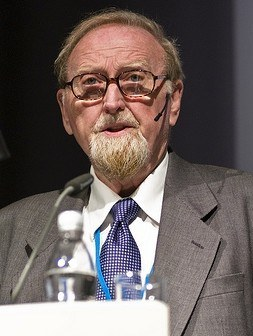
\includegraphics[height=0.40\textheight]{ch3_clive_granger_2008.jpg}\\[1mm]
\imgcap{Clive Granger (1934--2009)}
\imgcredit{https://commons.wikimedia.org/wiki/File:Clive_Granger_by_Olaf_Storbeck_(3x4_cropped).jpg}{Foto: Olaf Storbeck (2008); CC BY-SA 2.0; Wikimedia Commons}
\end{column}
\begin{column}{0.62\textwidth}
\centering
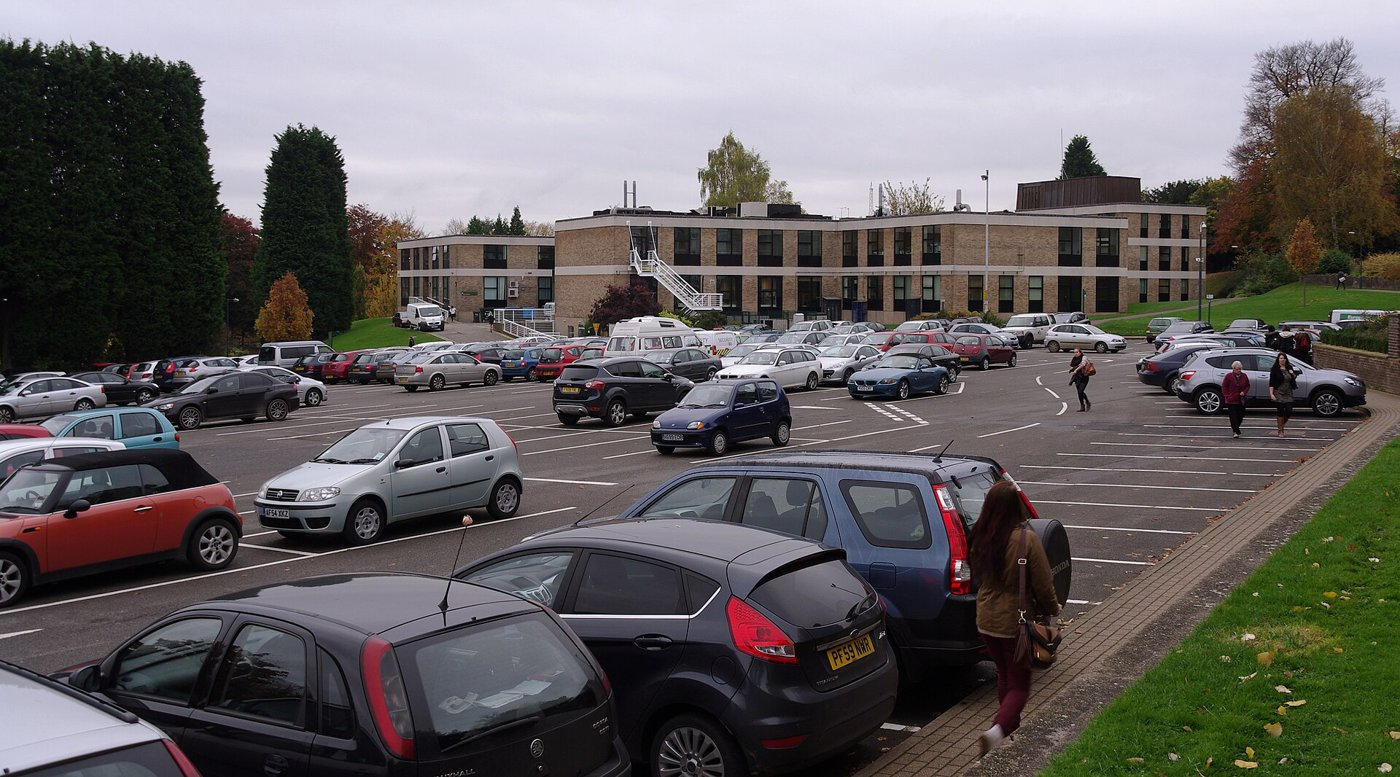
\includegraphics[height=0.30\textheight]{ch7_granger_building_2012.jpg}\\[1mm]
\imgcap{Clădirea Sir Clive Granger, Universitatea din Nottingham}
\imgcredit{https://commons.wikimedia.org/wiki/File:University_Park_MMB_\%C2\%AB24_Sir_Clive_Granger_Building.jpg}{Foto: mattbuck (2012); CC BY-SA 3.0; Wikimedia Commons}
\begin{itemize}
    \item Granger a studiat și și-a început cariera la Nottingham; cointegrarea a fost dezvoltată la UC San Diego
    \item Prelegerea Nobel: \refGrangerN: „time series analysis, cointegration, and applications”
\end{itemize}
\end{column}
\end{columns}
\end{frame}

\begin{frame}{Exemplu rezolvat: un VECM cu două variabile}
\itemsize{\small}
\begin{itemize}
    \item $\Delta y_{1t} = -0{,}10\,(y_{1,t-1} - y_{2,t-1}) + u_{1t}$, \quad $\Delta y_{2t} = 0{,}10\,(y_{1,t-1} - y_{2,t-1}) + u_{2t}$
    \begin{itemize}
        \item $\beta = (1, -1)^\top$, $\alpha = (-0{,}10; 0{,}10)^\top$; $\Pi = \alpha\beta^\top = \begin{pmatrix} -0{,}10 & 0{,}10 \\ 0{,}10 & -0{,}10 \end{pmatrix}$, $\det\Pi = 0$, rangul 1
    \end{itemize}
    \item Dacă $y_1$ este peste $y_2$: $y_1$ scade ($\alpha_1 < 0$), iar $y_2$ crește ($\alpha_2 > 0$): ambele închid distanța
    \item Distanța $z_t = y_{1t} - y_{2t}$: $z_t = (1 + \beta^\top\alpha)\,z_{t-1} + (u_{1t} - u_{2t}) = 0{,}8\,z_{t-1} + \dots$
    \begin{itemize}
        \item un AR(1) staționar; timpul de înjumătățire $\ln 0{,}5/\ln 0{,}8 = 3{,}1$ perioade; condiția este $-2 < \beta^\top\alpha < 0$
    \end{itemize}
    \item Media $(y_{1t} + y_{2t})/2$ variază cu $(u_{1t} + u_{2t})/2$: un mers aleator, trendul comun
\end{itemize}
\end{frame}

\begin{frame}{Termenii determiniști: cinci cazuri}
\itemsize{\small}
\begin{center}
\scriptsize
\begin{tabular}{>{\raggedright\arraybackslash}p{0.6cm}>{\raggedright\arraybackslash}p{4.6cm}>{\raggedright\arraybackslash}p{4.4cm}>{\raggedright\arraybackslash}p{2.6cm}}
\toprule
\textbf{Cazul} & \textbf{În VECM} & \textbf{Implicația pentru date} & \texttt{statsmodels} \\
\midrule
1 & fără constantă, fără trend & fără derivă; relații prin origine & \texttt{n} \\
2 & constantă doar în $\beta^\top\mathbf y_{t-1}$ & fără derivă; erori de echilibru cu medie nenulă (randamente, spread-uri) & \texttt{ci} \\
3 & constantă nerestricționată & trenduri liniare în niveluri, nu și în relații (PIB, prețuri) & \texttt{co} \\
4 & constantă și trend în $\beta^\top\mathbf y_{t-1}$ & trenduri în niveluri și în relații & \texttt{coli} \\
5 & constantă și trend nerestricționate & trenduri pătratice în niveluri; rareori plauzibil & \texttt{colo} \\
\bottomrule
\end{tabular}
\end{center}
\begin{itemize}
    \item Valorile critice ale testelor Johansen se schimbă de la un caz la altul \refJohBook; alegem cazul după grafic și după teorie, înainte de testare
    \item \texttt{coint\_johansen} din \texttt{statsmodels} implementează cazul 1 (\texttt{det\_order=-1}) și cazul 3 (\texttt{det\_order=0}), cazul folosit în acest capitol
\end{itemize}
\end{frame}

\begin{frame}{Exogenitatea slabă}
\itemsize{\small}
\begin{itemize}
    \item Dacă un rînd din $\alpha$ este nul, $\alpha_i = 0$, variabila $y_i$ \textbf{nu} reacționează la erorile de echilibru
    \begin{itemize}
        \item $y_i$ este \textbf{slab exogenă} pentru $\beta$: celelalte variabile fac toată ajustarea
        \item $y_i$ antrenează trendul comun; de exemplu Euribor pentru ratele dobînzii din România (Seminarul 7, B4)
    \end{itemize}
    \item Testul: un test $t$ pentru $\alpha_i$ (un vector de cointegrare) sau un test al raportului de verosimilitate (LR) pentru $\alpha_i = 0$ \refJohB
    \begin{itemize}
        \item statistica are asimptotic distribuția $\chi^2$ cu $r$ grade de libertate, după ce $r$ a fost fixat
    \end{itemize}
    \item Utilitate: dacă $x_t$ este slab exogenă, un ECM cu o singură ecuație pentru $y_t$ (secțiunea 3) nu pierde informație despre $\beta$
\end{itemize}
\end{frame}

\begin{frame}{Recapitulare: modelul VECM}
\itemsize{\small}
\begin{itemize}
    \item $\Delta\mathbf y_t = \alpha\beta^\top\mathbf y_{t-1} + \sum\Gamma_i\Delta\mathbf y_{t-i} + \mathbf u_t$: un VAR rescris; $\mathrm{rang}(\Pi) = r$
    \item Reprezentarea Granger: cointegrare $\Leftrightarrow$ corecția erorii; un VAR în diferențe omite termenul lung
    \item $\beta$: echilibre; $\alpha$: cine se ajustează; termenii determiniști: cinci cazuri; $\alpha_i = 0$: exogenitate slabă
\end{itemize}
\end{frame}


%=============================================================================
\section{Testele Johansen}
%=============================================================================

\begin{frame}{Ideea: regresia cu rang redus}
\itemsize{\small}
\begin{columns}[T]
\begin{column}{0.36\textwidth}
\centering
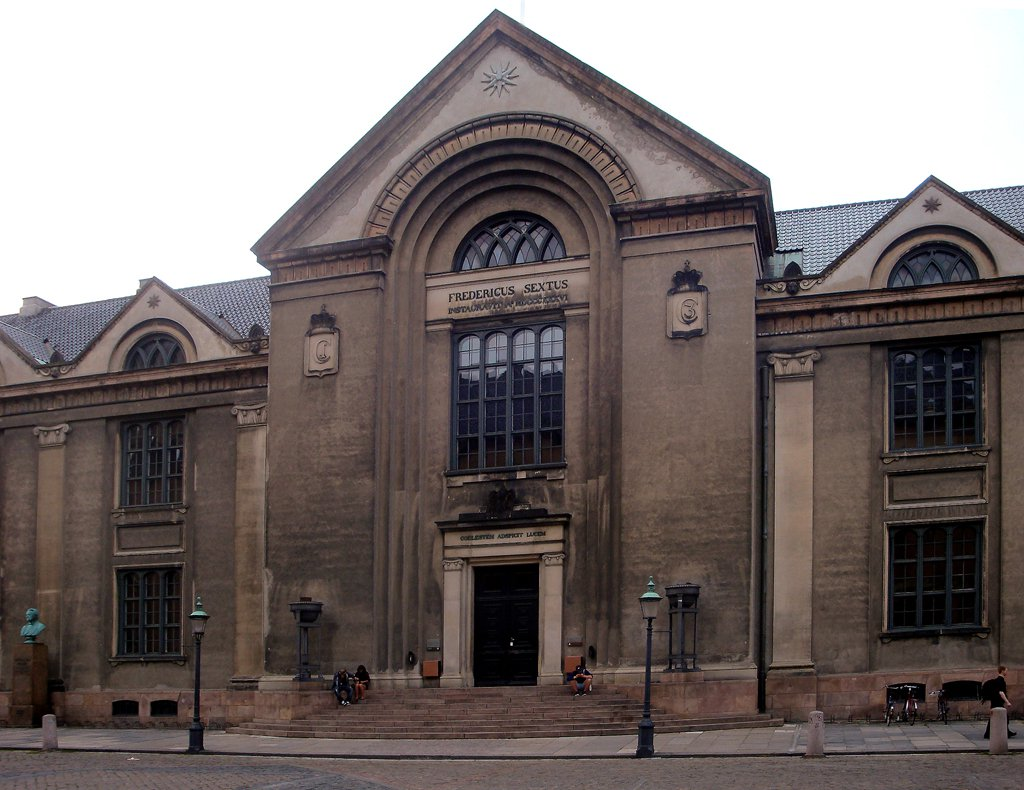
\includegraphics[height=0.36\textheight]{ch7_copenhagen_university_2011.jpg}\\[1mm]
\imgcap{Universitatea din Copenhaga, unde Søren Johansen și Katarina Juselius au dezvoltat metoda}
\imgcredit{https://commons.wikimedia.org/wiki/File:Copenhagen_University_Main_Entrance_DSC09700.jpg}{Foto: Per Meistrup (2011); CC BY-SA 4.0; Wikimedia Commons}
\end{column}
\begin{column}{0.60\textwidth}
\begin{itemize}
    \item \refJohA, \refJohB: verosimilitate maximă pentru VECM, cu erori gaussiene
    \begin{itemize}
        \item regresăm $\Delta\mathbf y_t$ și $\mathbf y_{t-1}$ pe diferențele decalate; păstrăm reziduurile $R_{0t}$ și $R_{1t}$
        \item căutăm combinațiile lui $R_{1t}$ cel mai puternic corelate cu $R_{0t}$: \textbf{corelațiile canonice}
    \end{itemize}
    \item Pătratele lor sînt valorile proprii $1 > \hat\lambda_1 \ge \dots \ge \hat\lambda_n \ge 0$
    \begin{itemize}
        \item un $\hat\lambda_i$ mare: o combinație staționară care prezice variațiile; $\hat\lambda_i \approx 0$: o combinație care rămîne $I(1)$
        \item vectorii proprii dau $\hat\beta$; apoi $\hat\alpha$ rezultă prin OLS
    \end{itemize}
\end{itemize}
\end{column}
\end{columns}
\end{frame}

\begin{frame}{Statisticile urmei și a valorii proprii maxime}
\itemsize{\small}
\begin{itemize}
    \item \textbf{Testul urmei}: $H_0$: rang $\le r$, față de rang $= n$; \quad $\lambda_{\mathrm{trace}}(r) = -T\sum_{i=r+1}^{n}\ln(1 - \hat\lambda_i)$
    \item \textbf{Testul valorii proprii maxime}: $H_0$: rang $= r$, față de rang $= r + 1$; \quad $\lambda_{\max}(r) = -T\ln(1 - \hat\lambda_{r+1})$
    \item \textbf{Procedura secvențială}: testăm $r = 0$, apoi $r \le 1$ etc.; rangul este primul $r$ pentru care $H_0$ \textbf{nu} este respinsă
    \begin{itemize}
        \item statisticile sînt rapoarte de verosimilitate, dar distribuțiile lor sînt nestandard (funcții de mișcări browniene)
        \item valorile critice depind de $n - r$ și de cazul termenilor determiniști: \refOL, \refMHM
    \end{itemize}
    \item Cele două teste concordă de obicei; dacă nu, în majoritatea lucrărilor aplicate se preferă testul urmei
\end{itemize}
\end{frame}

\begin{frame}{Exemplu rezolvat: de la valori proprii la statistici}
\itemsize{\small}
\begin{itemize}
    \item Randamentele din SUA la 1, 5 și 10 ani, lunar, $T = 801$: $\hat\lambda = (0{,}0405; 0{,}0229; 0{,}0039)$
    \begin{itemize}
        \item $-\ln(1 - \hat\lambda_i)$: 0{,}0414; 0{,}0231; 0{,}0039
    \end{itemize}
    \item $r = 0$: urma $= 801 \times (0{,}0414 + 0{,}0231 + 0{,}0039) = 54{,}8 > 29{,}80$: respingem
    \begin{itemize}
        \item valoarea proprie maximă: $801 \times 0{,}0414 = 33{,}2 > 21{,}13$: respingem
    \end{itemize}
    \item $r \le 1$: urma $= 21{,}7 > 15{,}49$: respingem; \quad $r \le 2$: urma $= 3{,}1 < 3{,}84$: nu respingem
    \begin{itemize}
        \item rangul 2: doi vectori de cointegrare, un singur trend comun
    \end{itemize}
    \item Și valorile proprii mici contează: sînt înmulțite cu $T$
\end{itemize}
\end{frame}

\begin{frame}{Testele Johansen pe trei sisteme}
\itemsize{\small}
\begin{center}
\scriptsize
\begin{tabular}{lrrcccccc}
\toprule
\textbf{Sistemul} & $T$ & $k$ & $\lambda_{\mathrm{trace}}(0)$ & $\lambda_{\mathrm{trace}}(1)$ & $\lambda_{\mathrm{trace}}(2)$ & $\lambda_{\max}(0)$ & $\lambda_{\max}(1)$ & \textbf{rang} \\
\midrule
SUA: randamentele la 1, 5 și 10 ani & 801 & 2 & 54{,}6 & 21{,}6 & 3{,}1 & 33{,}0 & 18{,}5 & 2 \\
SUA: PIB, consum, investiții & 203 & 1 & 28{,}9 & 11{,}4 & 2{,}6 & 17{,}4 & 8{,}9 & 0 \\
EUR/RON, EUR/HUF, EUR/PLN & 255 & 1 & 24{,}2 & 7{,}9 & 2{,}7 & 16{,}3 & 5{,}2 & 0 \\
Valoarea critică de 5\% & & & 29{,}80 & 15{,}49 & 3{,}84 & 21{,}13 & 14{,}26 & \\
\bottomrule
\end{tabular}
\end{center}
\begin{itemize}
    \item Cazul 3 (constantă nerestricționată); $k$: numărul de diferențe decalate, ales după BIC pentru VAR-ul în niveluri; rangurile după testul urmei (testul valorii proprii maxime dă aici aceleași ranguri)
    \item Randamentele: FRED, 1960--2026; PIB, consum și investiții: 100 ln, SUA 1959--2009; monedele: BNR, sfîrșitul lunii, 2005--2026
\end{itemize}
\end{frame}

\begin{frame}{Interpretarea celor trei sisteme}
\itemsize{\small}
\begin{itemize}
    \item Randamentele: rangul 2, deci un singur trend comun: \textbf{nivelul} ratelor mișcă toate scadențele; cele două spread-uri sînt staționare
    \begin{itemize}
        \item ipoteza așteptărilor pentru structura la termen \refCS, în forma ei slabă
    \end{itemize}
    \item PIB, consum și investiții: urma 28{,}9 față de 29{,}80: rangul 0 la 5\%, foarte aproape de respingere
    \begin{itemize}
        \item creșterea echilibrată prezice rangul 2 (ponderi stabile ale consumului și investițiilor); cu Engle--Granger, consumul și venitul erau cointegrate (p = 0{,}029): putere mică, nu dovada absenței
    \end{itemize}
    \item Monedele: urma 24{,}2: rangul 0; trei trenduri stochastice separate (secțiunea 8)
\end{itemize}
\end{frame}

\begin{frame}{Cazul termenilor determiniști schimbă răspunsul}
\itemsize{\small}
\begin{center}
\scriptsize
\begin{tabular}{lcccccc}
\toprule
\textbf{Termeni determiniști} & $\lambda_{\mathrm{trace}}(0)$ & 5\% & $\lambda_{\mathrm{trace}}(1)$ & 5\% & $\lambda_{\mathrm{trace}}(2)$ & 5\% \\
\midrule
niciunul (\texttt{det\_order=-1}) & 45{,}9 & 24{,}28 & 13{,}3 & 12{,}32 & 0{,}4 & 4{,}13 \\
constantă (\texttt{det\_order=0}) & 54{,}6 & 29{,}80 & 21{,}6 & 15{,}49 & 3{,}1 & 3{,}84 \\
trend liniar (\texttt{det\_order=1}) & 60{,}0 & 35{,}01 & 23{,}7 & 18{,}40 & 4{,}8 & 3{,}84 \\
\bottomrule
\end{tabular}
\end{center}
\begin{itemize}
    \item Randamentele din SUA la 1, 5 și 10 ani: rangurile 2, 2 și 3
    \item Cu trend liniar, testul spune că fiecare randament este staționar în jurul unui trend: neplauzibil pentru ratele dobînzii pe 66 de ani
    \begin{itemize}
        \item alegem termenii determiniști după teorie și după grafic, nu după rezultatul care ne convine
    \end{itemize}
    \item Alte probleme practice: numărul de decalaje $k$; distorsiunile nivelului de semnificație în eșantioane mici (factorul de corecție $(T - nk)/T$, \refRA); rupturile structurale
\end{itemize}
\end{frame}

\begin{frame}{Studiu de caz: Johansen și Juselius (1990)}
\itemsize{\small}
\begin{itemize}
    \item \textbf{Întrebarea}: există o cerere de bani stabilă în Danemarca și Finlanda?
    \begin{itemize}
        \item \refJJ: masa monetară reală, venitul real, ratele dobînzii (și inflația); date trimestriale
    \end{itemize}
    \item \textbf{Metoda}: VECM prin verosimilitate maximă; rangul prin testele urmei și ale valorii proprii maxime; apoi \textbf{teste ale restricțiilor} asupra lui $\beta$ și $\alpha$
    \begin{itemize}
        \item de exemplu o elasticitate unitară față de venit, $\beta = (1, -1, \cdot)$; exogenitatea slabă a venitului și a ratelor dobînzii
    \end{itemize}
    \item \textbf{Moștenirea}: modelul metodologiei „VAR cointegrat” \refJus: testăm rangul, apoi testăm ipotezele economice ca restricții
    \begin{itemize}
        \item una dintre cele mai citate lucrări din econometria aplicată
    \end{itemize}
\end{itemize}
\end{frame}

\begin{frame}{Recapitulare: testele Johansen}
\itemsize{\small}
\begin{itemize}
    \item Valorile proprii ale unei regresii cu rang redus; statisticile urmei și a valorii proprii maxime; testare secvențială de la $r = 0$
    \item Valorile critice depind de $n - r$ și de cazul termenilor determiniști
    \item Randamentele: rangul 2; agregatele macroeconomice: la limită; monedele: rangul 0
\end{itemize}
\end{frame}


%=============================================================================
\section{Estimarea și interpretarea lui $\beta$ și $\alpha$}
%=============================================================================

\begin{frame}{Modelul VECM al structurii la termen}
\itemsize{\footnotesize}
\begin{center}
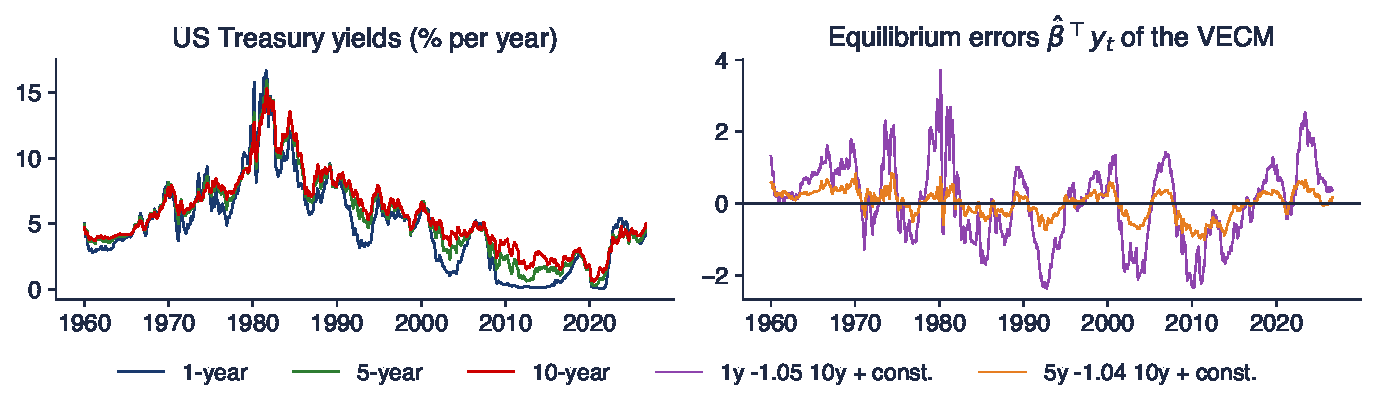
\includegraphics[width=0.97\textwidth,height=0.55\textheight,keepaspectratio]{tsa_ch7_rates.pdf}
\end{center}
\vspace{-0.25cm}
\begin{itemize}
    \item Randamentele titlurilor de stat americane la 1, 5 și 10 ani (FRED GS1, GS5, GS10), ianuarie 1960--septembrie 2026; VECM cu rangul 2, 2 diferențe decalate, constantă restricționată la relații (cazul 2)
\end{itemize}
\quantlet{TSA\_ch7\_johansen\_vecm}{\qlurl{TSA_ch7_johansen_vecm}}
\end{frame}

\begin{frame}{Interpretarea vectorilor de cointegrare}
\itemsize{\small}
\begin{itemize}
    \item Normalizare pe randamentele la 1 și 5 ani: $\hat\beta_1^\top\mathbf y_t = i^{(1)}_t - 1{,}045\,i^{(10)}_t + 1{,}22$, $\hat\beta_2^\top\mathbf y_t = i^{(5)}_t - 1{,}044\,i^{(10)}_t + 0{,}59$
    \begin{itemize}
        \item ambele pante sînt apropiate de 1: echilibrele sînt aproape spread-urile $i^{(1)} - i^{(10)}$ și $i^{(5)} - i^{(10)}$, cu prime de termen medii
    \end{itemize}
    \item Erorile de echilibru sînt staționare: ADF p $<$\,0{,}001 și 0{,}008; sînt mari în anii 1980 și în perioadele cu dobînzi aproape de zero
    \item Un test formal pentru $\beta = (1, -1)$ la fiecare spread este un test al raportului de verosimilitate \refJohB; cu $\hat\beta$ superconsistent, valori atît de apropiate de 1 sînt informative
\end{itemize}
\end{frame}

\begin{frame}{Coeficienții de ajustare}
\itemsize{\small}
\begin{center}
\footnotesize
\begin{tabular}{lcccc}
\toprule
\textbf{Ecuația} & $\hat\alpha_{\cdot 1}$ & $t$ & $\hat\alpha_{\cdot 2}$ & $t$ \\
\midrule
$\Delta i^{(1)}_t$ (1 an) & $-0{,}021$ & $-0{,}82$ & $0{,}024$ & $0{,}31$ \\
$\Delta i^{(5)}_t$ (5 ani) & $0{,}045$ & $2{,}21$ & $-0{,}122$ & $-2{,}00$ \\
$\Delta i^{(10)}_t$ (10 ani) & $0{,}040$ & $2{,}22$ & $-0{,}077$ & $-1{,}43$ \\
\bottomrule
\end{tabular}
\end{center}
\begin{itemize}
    \item Randamentul la 1 an nu reacționează la niciuna dintre erori ($|t| < 1$): se comportă ca \textbf{slab exogen}
    \begin{itemize}
        \item capătul scurt urmează politica monetară; randamentele la 5 și 10 ani fac ajustarea ($|t| \approx 2$)
    \end{itemize}
    \item Erorile de echilibru urmează $\mathbf z_t = (I + \hat\beta^\top\hat\alpha)\,\mathbf z_{t-1} + \dots$; valorile proprii 0{,}969 și 0{,}926
    \begin{itemize}
        \item timpi de înjumătățire de circa 22{,}1 și 9{,}0 luni: corecție lentă a erorii, tipică pentru ratele dobînzii
    \end{itemize}
\end{itemize}
\end{frame}

\begin{frame}{Funcțiile de răspuns la impuls ale modelului VECM}
\itemsize{\footnotesize}
\begin{center}
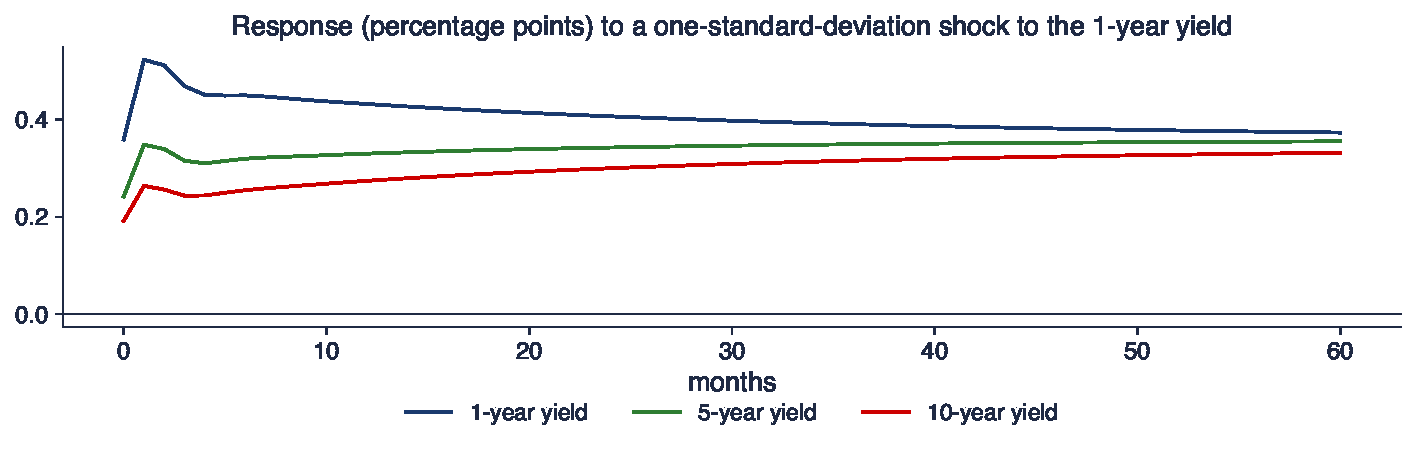
\includegraphics[width=0.97\textwidth,height=0.50\textheight,keepaspectratio]{tsa_ch7_vecm_irf.pdf}
\end{center}
\vspace{-0.25cm}
\begin{itemize}
    \item Răspunsuri ortogonalizate (Cholesky, ordinea 1 an, 5 ani, 10 ani; \tsachlink{https://danpele.github.io/Time-Series-Analysis/RO/Cursuri/capitol6_modele_var_cauzalitate_granger.pdf}{Capitolul 6}) la un șoc de o abatere standard asupra randamentului la 1 an
\end{itemize}
\quantlet{TSA\_ch7\_johansen\_vecm}{\qlurl{TSA_ch7_johansen_vecm}}
\end{frame}

\begin{frame}{Interpretarea răspunsurilor la impuls}
\itemsize{\small}
\begin{itemize}
    \item La impact: +0{,}36, +0{,}24 și +0{,}19 puncte procentuale pentru 1, 5 și 10 ani
    \begin{itemize}
        \item după 60 de luni: +0{,}37, +0{,}36 și +0{,}33: efectele \textbf{nu} se sting și devin aproape egale
    \end{itemize}
    \item O deplasare permanentă a trendului comun (nivelul), cu spread-uri staționare: semnătura unui singur trend comun, $n - r = 1$
    \item Într-un VAR staționar (\tsachlink{https://danpele.github.io/Time-Series-Analysis/RO/Cursuri/capitol6_modele_var_cauzalitate_granger.pdf}{Capitolul 6}) orice răspuns revine la zero; într-un VECM, răspunsurile pe termen lung sînt în general diferite de zero
\end{itemize}
\end{frame}

\begin{frame}{Recapitulare: $\beta$ și $\alpha$}
\itemsize{\small}
\begin{itemize}
    \item $\hat\beta$: normalizăm, interpretăm ca echilibre (spread-uri, rapoarte), testăm restricțiile economice
    \item $\hat\alpha$: cine se ajustează și cît de repede; un rînd nul înseamnă exogenitate slabă
    \item Șocurile au efecte permanente asupra nivelurilor cointegrate, dar nu asupra erorilor de echilibru
\end{itemize}
\end{frame}


%=============================================================================
\section{Prognoza: VECM sau VAR în diferențe?}
%=============================================================================

\begin{frame}{Argumentele teoretice}
\itemsize{\small}
\begin{itemize}
    \item Prognozele VECM păstrează echilibrele: pe măsură ce orizontul crește, $\hat\beta^\top\hat{\mathbf y}_{T+h}$ revine la media sa
    \begin{itemize}
        \item un VAR în diferențe uită nivelurile: prognozele lui pentru spread-uri rămîn unde se află
    \end{itemize}
    \item \refEY: impunerea cointegrării îmbunătățește prognozele pe orizonturi lungi în sisteme simulate
    \item \refCD: cîștigurile sînt concentrate în \textbf{combinațiile de cointegrare}
    \begin{itemize}
        \item pentru nivelurile individuale, eroarea de prognoză este dominată de trendul comun, pe care niciun model nu îl poate prezice
        \item eroarea de estimare din $\alpha$, $\beta$ și din constante poate face un VECM mai slab în practică
    \end{itemize}
    \item Verificăm în afara eșantionului, cu reestimare la fiecare origine a prognozei
\end{itemize}
\end{frame}

\begin{frame}{Experimentul de prognoză}
\itemsize{\small}
\begin{itemize}
    \item Datele: randamentele din SUA la 1, 5 și 10 ani, lunar, din 1960
    \item 135 de origini ale prognozei, la fiecare trei luni, din ianuarie 1990 pînă în iulie 2023; modelele sînt reestimate pe datele de pînă la fiecare origine
    \begin{itemize}
        \item VECM cu rangul 2 și constantă restricționată; VAR în diferențe fără constantă, cu aceleași decalaje; mersul aleator (fără schimbare)
    \end{itemize}
    \item Orizonturi de la 1 la 36 de luni; RMSE (root mean squared error, rădăcina erorii pătratice medii) a fiecărui model împărțită la cea a mersului aleator
    \begin{itemize}
        \item raport sub 1: mai bun decît mersul aleator; și pentru spread-ul dintre randamentul la 10 ani și cel la 1 an
    \end{itemize}
\end{itemize}
\end{frame}

\begin{frame}{VECM față de un VAR în diferențe, în afara eșantionului}
\itemsize{\footnotesize}
\begin{center}
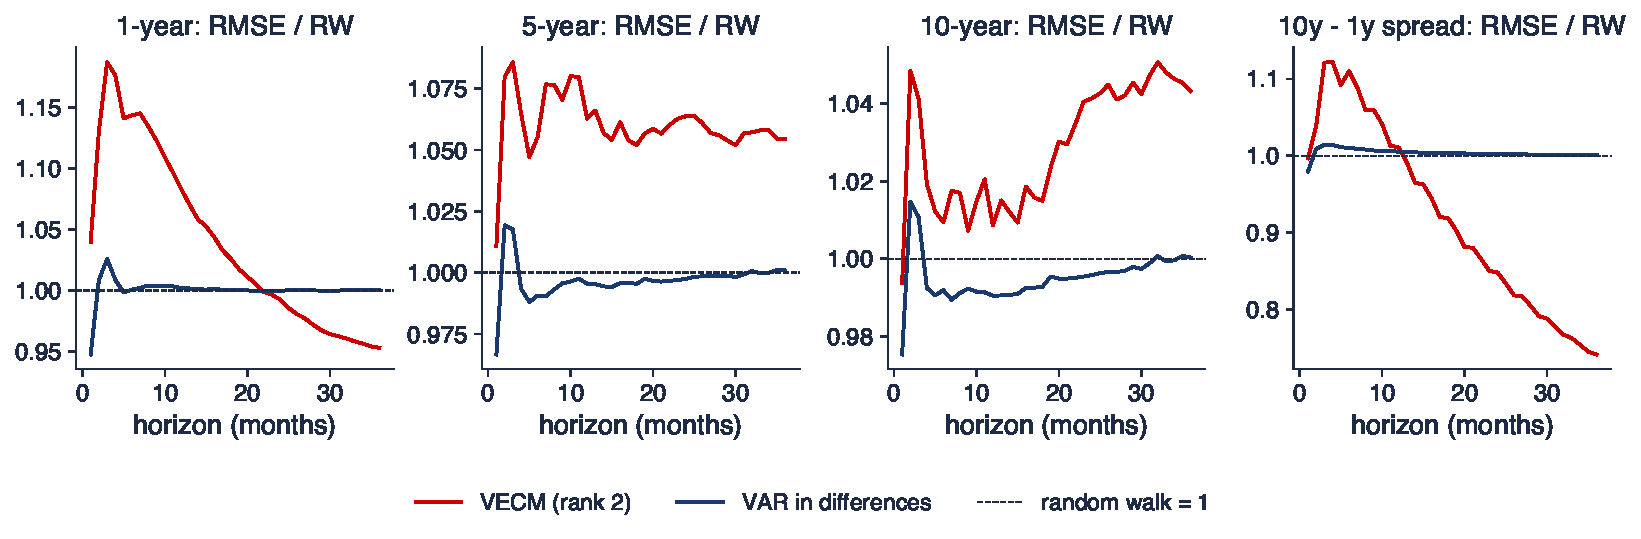
\includegraphics[width=0.97\textwidth,height=0.52\textheight,keepaspectratio]{tsa_ch7_forecast.pdf}
\end{center}
\vspace{-0.25cm}
\begin{itemize}
    \item RMSE relativ la mersul aleator, pe orizonturi; primele trei panouri: randamentele; ultimul panou: spread-ul 10 ani minus 1 an
\end{itemize}
\quantlet{TSA\_ch7\_forecasting}{\qlurl{TSA_ch7_forecasting}}
\end{frame}

\begin{frame}{Interpretarea comparației prognozelor}
\itemsize{\small}
\begin{itemize}
    \item Nivelurile: niciun model nu bate clar mersul aleator; VECM este mai slab pe orizonturi scurte (1 an la 6 luni: 1{,}14; 5 ani: 1{,}06)
    \begin{itemize}
        \item VAR-ul în diferențe rămîne aproape de 1 la orice orizont (1 an la 12 luni: 1{,}00)
    \end{itemize}
    \item Spread-ul: VECM cîștigă pe orizonturi lungi: 0{,}85 la 24 de luni și 0{,}74 la 36 de luni; VAR-ul în diferențe: 1{,}00
    \begin{itemize}
        \item exact tiparul din \refCD: cointegrarea ajută la prognoza erorilor de echilibru, nu a trendului
    \end{itemize}
    \item Lecția: folosim un VECM cînd ne interesează relația (un spread, un raport, o pereche); pentru nivelurile singure, mersul aleator este greu de depășit
\end{itemize}
\end{frame}

\begin{frame}{Recapitulare: prognoza}
\itemsize{\small}
\begin{itemize}
    \item VECM readuce prognozele erorilor de echilibru la mediile lor; VAR-ul în diferențe nu face acest lucru
    \item În afara eșantionului: cîștiguri pentru spread pe orizonturi lungi, niciunul pentru niveluri
    \item Comparăm întotdeauna cu mersul aleator, cu reestimare și fără a folosi date din viitor
\end{itemize}
\end{frame}


%=============================================================================
\section{Exemple economice: paritate și rate ale dobînzii}
%=============================================================================

\begin{frame}{Paritatea puterii de cumpărare}
\itemsize{\small}
\begin{columns}[T]
\begin{column}{0.34\textwidth}
\centering

\includegraphics[height=0.34\textheight]{ch7_bnr_palace_2015.jpg}\\[1mm]
\imgcap{Banca Națională a României, care publică cursurile de referință}
\imgcredit{https://commons.wikimedia.org/wiki/File:Bucharest_-_BNR_Palace_(19644434340).jpg}{Foto: Ștefan Jurcă (2015); CC BY 2.0; Wikimedia Commons}
\end{column}
\begin{column}{0.62\textwidth}
\begin{itemize}
    \item \textbf{Paritatea relativă a puterii de cumpărare} (PPP, purchasing power parity): cursul compensează diferențele de inflație
    \begin{itemize}
        \item $s_t = 100\ln(\mathrm{EUR/RON})$; $p_t$, $p^*_t$: $100\ln$ din IAPC (indicele armonizat al prețurilor de consum) al României și al zonei euro
        \item PPP este valabilă pe termen lung dacă cursul real $q_t = s_t - p_t + p^*_t$ este staționar: cointegrare cu $\beta = (1, -1, 1)$
    \end{itemize}
    \item De ce poate să nu fie valabilă
    \begin{itemize}
        \item \refBalassa: creșterea rapidă a productivității în sectorul bunurilor comercializabile ridică prețurile serviciilor necomercializabile într-o economie în convergență: o apreciere reală în trend
        \item chiar acolo unde PPP este valabilă, abaterile se sting lent; sinteza \refTT\ raportează timpi de înjumătățire de mai mulți ani
    \end{itemize}
\end{itemize}
\end{column}
\end{columns}
\end{frame}

\begin{frame}{PPP pentru leu}
\itemsize{\footnotesize}
\begin{center}
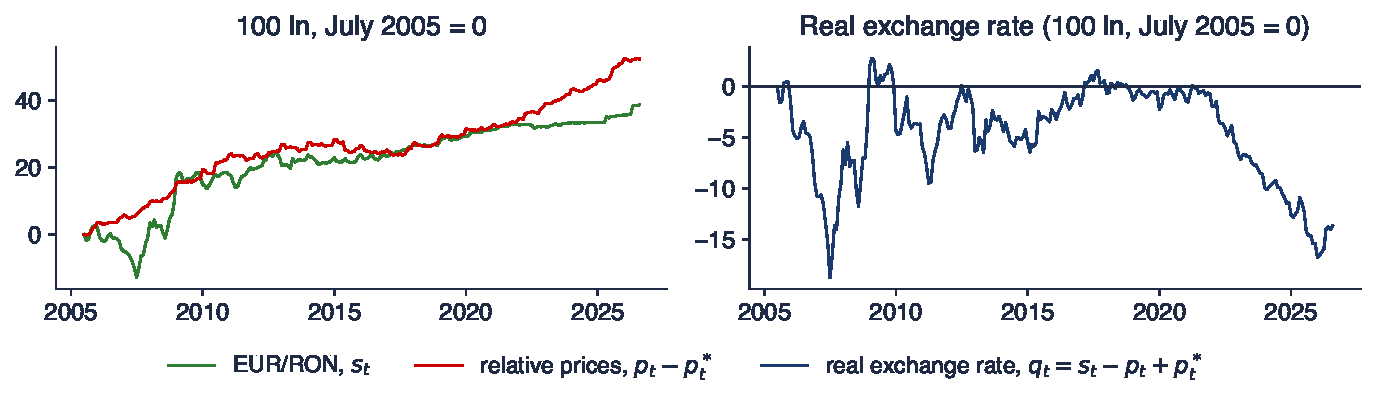
\includegraphics[width=0.97\textwidth,height=0.55\textheight,keepaspectratio]{tsa_ch7_ppp.pdf}
\end{center}
\vspace{-0.25cm}
\begin{itemize}
    \item Lunar, iulie 2005--august 2026: EUR/RON (media lunară a cursului de referință BNR), IAPC al României și al zonei euro (Eurostat, 2015 = 100)
\end{itemize}
\quantlet{TSA\_ch7\_parity\_conditions}{\qlurl{TSA_ch7_parity_conditions}}
\end{frame}

\begin{frame}{Interpretarea PPP pentru leu}
\itemsize{\small}
\begin{itemize}
    \item Din 2005 leul a pierdut 38{,}7 puncte logaritmice față de euro, în timp ce prețurile din România au crescut cu 52{,}4 puncte logaritmice mai mult decît cele din zona euro
    \begin{itemize}
        \item cursul real s-a modificat cu $-13{,}7$ puncte logaritmice: o apreciere reală a leului, concentrată după 2021
    \end{itemize}
    \item ADF pe $q_t$: p = 0{,}24; Engle--Granger pentru $s_t$ pe $p_t - p^*_t$: panta 0{,}89, p = 0{,}34; Johansen pe $(s_t, p_t, p^*_t)$: rangul 0
    \item Nicio dovadă de PPP în 21 de ani, în acord cu convergența de tip Balassa--Samuelson; 21 de ani pot fi și prea puțini pentru timpi de înjumătățire de mai mulți ani
\end{itemize}
\end{frame}

\begin{frame}{ROBOR și Euribor}
\itemsize{\footnotesize}
\begin{center}
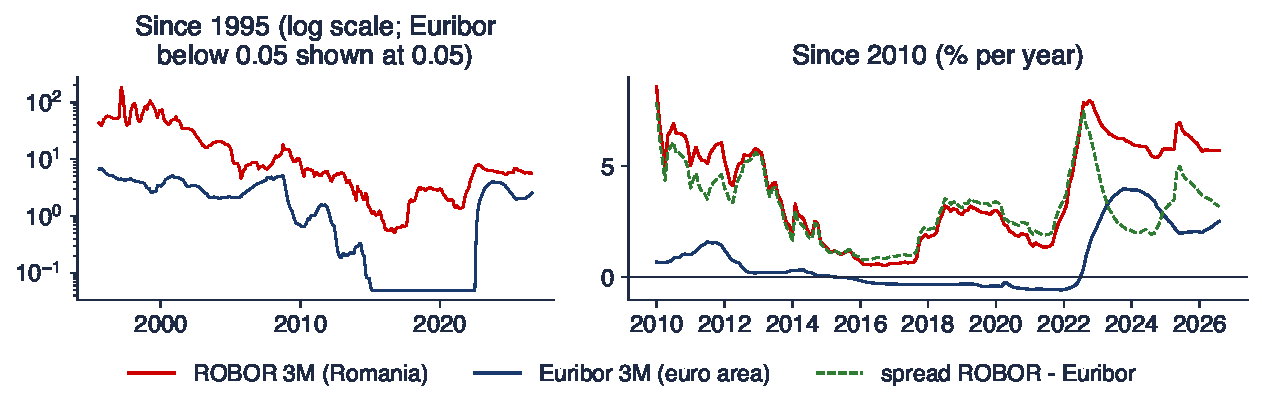
\includegraphics[width=0.97\textwidth,height=0.55\textheight,keepaspectratio]{tsa_ch7_ro_ea_rates.pdf}
\end{center}
\vspace{-0.25cm}
\begin{itemize}
    \item Ratele dobînzii pe piața monetară la trei luni (Eurostat), august 1995--august 2026: ROBOR 3M pentru România și Euribor 3M pentru zona euro
\end{itemize}
\quantlet{TSA\_ch7\_parity\_conditions}{\qlurl{TSA_ch7_parity_conditions}}
\end{frame}

\begin{frame}{Interpretarea ROBOR și Euribor}
\itemsize{\small}
\begin{itemize}
    \item Eșantionul complet: Engle--Granger p = 0{,}52, Phillips--Ouliaris p 0{,}010: dezinflația din anii 1990 domină, iar testele nu concordă
    \item Din 2010: p = 0{,}047 (Engle--Granger) și 0{,}029 (Phillips--Ouliaris), panta 1{,}19, spread-ul mediu 3{,}11 puncte procentuale
    \begin{itemize}
        \item ECM pentru ROBOR: $\hat\gamma = -0{,}020$ ($t = -1{,}18$), timp de înjumătățire de circa 34 de luni: ajustare slabă și lentă
    \end{itemize}
    \item Politica monetară a României urmărește propria țintă de inflație; legătura cu Euribor este slabă (Seminarul 7, B4, adaugă randamentul la 10 ani al României)
\end{itemize}
\end{frame}

\begin{frame}{Trei monede central-europene}
\itemsize{\footnotesize}
\begin{center}
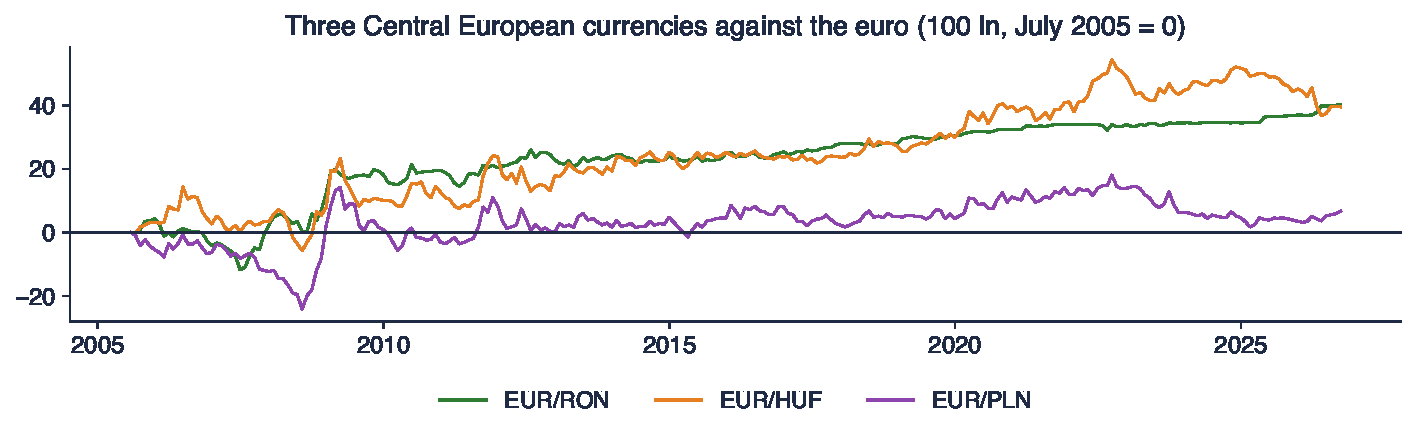
\includegraphics[width=0.97\textwidth,height=0.55\textheight,keepaspectratio]{tsa_ch7_cee_fx.pdf}
\end{center}
\vspace{-0.25cm}
\begin{itemize}
    \item EUR/RON, EUR/HUF și EUR/PLN, cursuri încrucișate calculate din cursurile de referință BNR, la sfîrșitul lunii, 100 ln
\end{itemize}
\quantlet{TSA\_ch7\_parity\_conditions}{\qlurl{TSA_ch7_parity_conditions}}
\end{frame}

\begin{frame}{Interpretarea celor trei monede}
\itemsize{\small}
\begin{itemize}
    \item Din iulie 2005: EUR/RON +40{,}1, EUR/HUF +39{,}5, EUR/PLN +6{,}7 puncte logaritmice; fiecare curs este $I(1)$ (ADF p = 0{,}55; 0{,}75; 0{,}08)
    \item Johansen: urma 24{,}2 pentru $r = 0$ (valoarea critică 29{,}80); nici din 2012 nu există cointegrare (urma 12{,}7)
    \begin{itemize}
        \item o ancoră comună (euro) și șocuri similare nu creează un trend comun: fiecare bancă centrală și fiecare evoluție a inflației adaugă propriul trend
    \end{itemize}
    \item Modelul potrivit pentru aceste cursuri este un VAR în diferențe (\tsachlink{https://danpele.github.io/Time-Series-Analysis/RO/Cursuri/capitol6_modele_var_cauzalitate_granger.pdf}{Capitolul 6}); Seminarul 7 (B3) reia analiza
\end{itemize}
\end{frame}

\begin{frame}{Recapitulare: exemple economice}
\itemsize{\small}
\begin{itemize}
    \item PPP pentru leu este respinsă în 2005--2026: aprecierea reală a unei economii în convergență
    \item ROBOR și Euribor: o legătură slabă și lentă din 2010; eșantionul decide verdictul
    \item Teoria propune $\beta$; testele, eșantionul și termenii determiniști decid dacă datele sînt de acord
\end{itemize}
\end{frame}


%=============================================================================
\section{O aplicație: pairs trading}
%=============================================================================

\begin{frame}{Ideea de pairs trading}
\itemsize{\small}
\begin{itemize}
    \item Două acțiuni expuse acelorași șocuri (două bănci, două companii petroliere) pot fi cointegrate: spread-ul lor revine la medie
    \begin{itemize}
        \item cînd spread-ul este neobișnuit de mare, vindem acțiunea scumpă și cumpărăm acțiunea ieftină; închidem cînd spread-ul a revenit
    \end{itemize}
    \item O tranzacție de \textbf{valoare relativă}: direcția pieței se anulează; profitul vine din corecția erorii
    \begin{itemize}
        \item \refGGR: metoda distanței pe acțiuni americane, profitabilă în perioada 1962--2002
        \item \refDoFaff: profiturile au scăzut în anii următori
    \end{itemize}
    \item Un bun test pentru o idee din seriile de timp: trebuie să funcționeze \textbf{în afara eșantionului}, \textbf{după costuri} și pe perechi alese \textbf{fără a privi în viitor}
\end{itemize}
\end{frame}

\begin{frame}{O regulă fără informații din viitor}
\itemsize{\small}
\begin{itemize}
    \item \textbf{Formarea} (cele 252 de zile de tranzacționare anterioare): testăm fiecare pereche cu Engle--Granger; păstrăm perechile cu p $<$ 0,05
    \begin{itemize}
        \item raportul de acoperire $\hat b$ prin OLS pentru $\ln P_A$ pe $\ln P_B$; media $\bar s$ și abaterea standard $\hat\sigma_s$ ale spread-ului $s_t = \ln P_{A,t} - \hat a - \hat b\ln P_{B,t}$
    \end{itemize}
    \item \textbf{Tranzacționarea} (următoarele 126 de zile), cu parametrii din formare ficși: $z_t = (s_t - \bar s)/\hat\sigma_s$
    \begin{itemize}
        \item $z_t > 2$: vindem A în lipsă, cumpărăm $\hat b$ din B; $z_t < -2$: invers; închidem la $z_t = 0$ sau la sfîrșitul ferestrei
        \item randamentul zilnic pe unitatea de expunere brută: $\pm(r_A - \hat b\,r_B)/(1 + |\hat b|)$; capital egal pentru fiecare pereche selectată
    \end{itemize}
    \item \textbf{Costuri}: 0{,}20\% (București) și 0{,}05\% (SUA) din expunerea brută tranzacționată, la fiecare deschidere și închidere
\end{itemize}
\end{frame}

\begin{frame}{Banca Transilvania și BRD}
\itemsize{\footnotesize}
\begin{center}
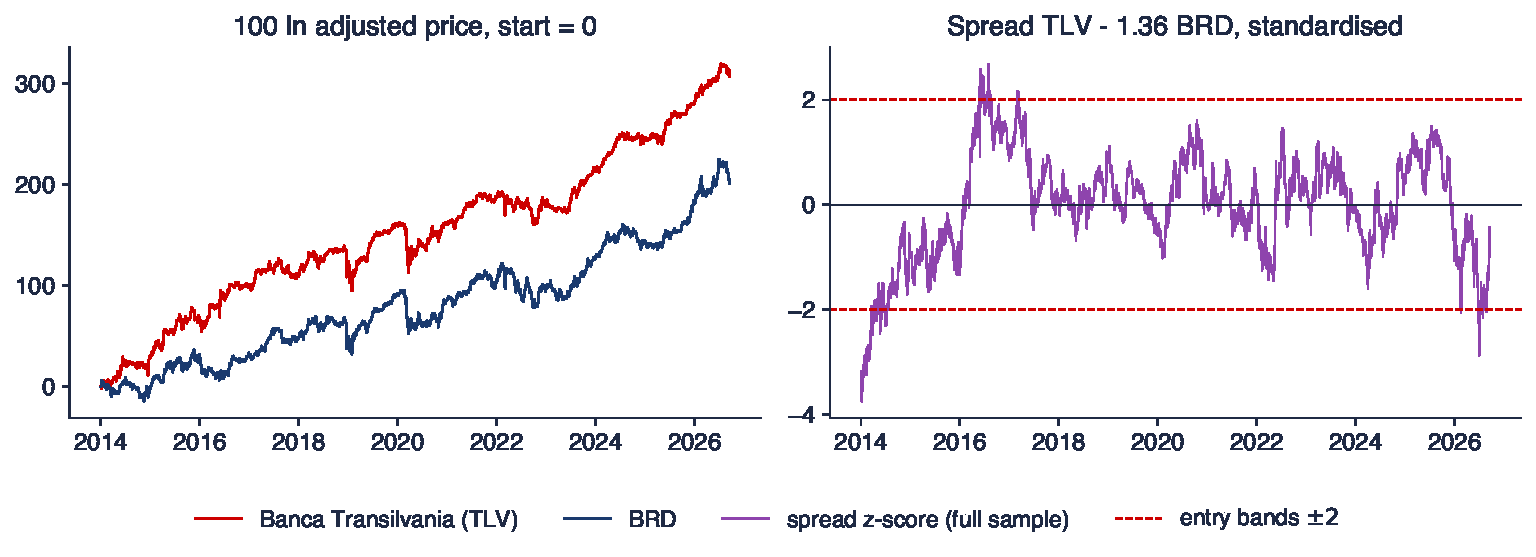
\includegraphics[width=0.97\textwidth,height=0.55\textheight,keepaspectratio]{tsa_ch7_pair.pdf}
\end{center}
\vspace{-0.25cm}
\begin{itemize}
    \item Prețuri zilnice ajustate din 2014; dreapta: spread-ul regresiei pe întregul eșantion, standardizat, cu benzile de intrare
\end{itemize}
\quantlet{TSA\_ch7\_pairs\_trading}{\qlurl{TSA_ch7_pairs_trading}}
\end{frame}

\begin{frame}{Interpretarea perechii de bănci}
\itemsize{\small}
\begin{itemize}
    \item Întregul eșantion: $\hat b = 1{,}36$; spread-ul este un AR(1) cu $\hat\rho = 0{,}990$: timp de înjumătățire de circa 69 de zile de tranzacționare
    \begin{itemize}
        \item doar 5{,}0\% din zile se află în afara benzii $\pm 2$: puține ocazii de tranzacționare, fiecare durînd luni de zile
    \end{itemize}
    \item Aplicarea regulii pe acest grafic, cu parametrii din întregul eșantion, dă 3{,}32\% pe an (raportul Sharpe 0{,}44), după costuri
    \begin{itemize}
        \item o iluzie: $\hat b$, $\bar s$ și $\hat\sigma_s$ folosesc viitorul, iar perechea a fost aleasă pentru că pare cointegrată din 2014
    \end{itemize}
    \item Cu regula pe ferestre mobile, perechea nu trece testul de formare în niciuna dintre cele 24 de ferestre: un an de date este prea puțin pentru a detecta o corecție atît de lentă
\end{itemize}
\end{frame}

\begin{frame}{Pairs trading în afara eșantionului}
\itemsize{\footnotesize}
\begin{center}
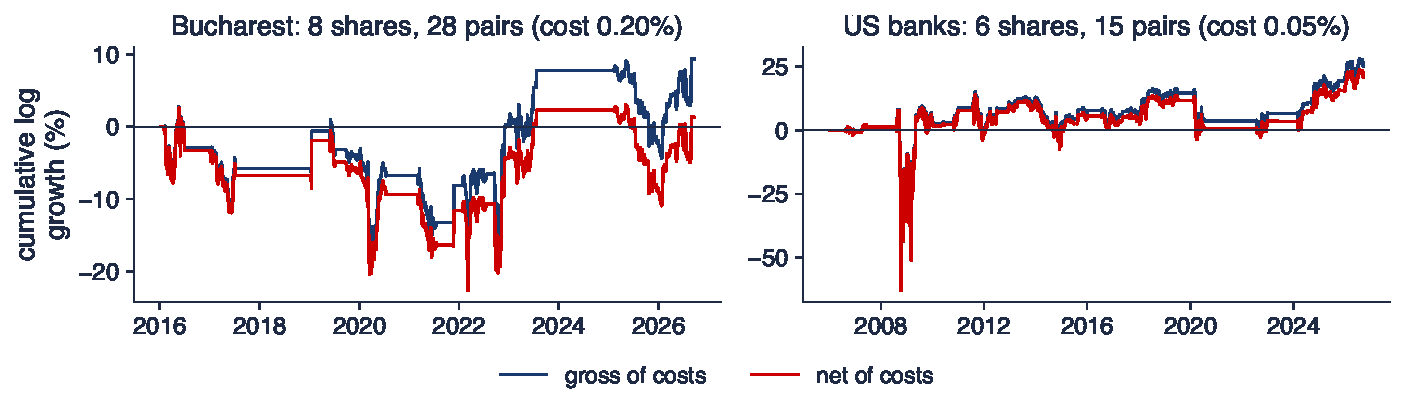
\includegraphics[width=0.97\textwidth,height=0.55\textheight,keepaspectratio]{tsa_ch7_pairs_backtest.pdf}
\end{center}
\vspace{-0.25cm}
\begin{itemize}
    \item Stînga: 8 acțiuni lichide de la BVB (TLV, BRD, SNP, TGN, TEL, EL, SNG, SNN), din 2015; dreapta: 6 bănci americane (JPM, BAC, C, WFC, GS, MS), din 2005
\end{itemize}
\quantlet{TSA\_ch7\_pairs\_trading}{\qlurl{TSA_ch7_pairs_trading}}
\end{frame}

\begin{frame}{Interpretarea testului istoric}
\itemsize{\small}
\begin{itemize}
    \item București: 22 de ferestre, perechi găsite în 14, 73 de tranzacții, 62\% dintre ele profitabile, dar randamentul mediu pe tranzacție este $-0{,}26$\%
    \begin{itemize}
        \item brut 1{,}17\% pe an (Sharpe 0{,}15); net 0{,}41\% (Sharpe 0{,}05); costul la care profitul net devine zero: 0{,}31\%
    \end{itemize}
    \item Băncile americane: brut 2{,}77\% (Sharpe 0{,}16), net 2{,}57\% (Sharpe 0{,}14), 80 de tranzacții
    \begin{itemize}
        \item cu o pierdere mare în toamna lui 2008: cointegrarea se poate rupe exact cînd contează
    \end{itemize}
    \item Multe cîștiguri mici și cîteva pierderi mari: profilul tipic al unei strategii de revenire la medie
\end{itemize}
\end{frame}

\begin{frame}{Capcanele pairs trading}
\itemsize{\small}
\begin{itemize}
    \item \textbf{Testarea multiplă}: cu 28 de perechi și un test de 5\%, circa 1{,}4 perechi trec întîmplător în fiecare fereastră
    \item \textbf{Informațiile din viitor}: alegerea perechilor, a datelor de început sau a pragurilor după ce am văzut întregul eșantion
    \item \textbf{Rupturile}: fuziunile, recapitalizările, reglementările și crizele schimbă $\beta$; spread-ul poate să nu mai revină
    \item \textbf{Fricțiunile pieței}: vînzarea în lipsă este limitată la BVB, împrumutul acțiunilor costă un comision, diferențele bid-ask sînt mari pentru companiile mici
    \item \textbf{Corecția lentă a erorii}: timpi de înjumătățire de luni înseamnă capital blocat luni de zile și o așteptare lungă într-o poziție pierzătoare
\end{itemize}
\end{frame}

\begin{frame}{Recapitulare: pairs trading}
\itemsize{\small}
\begin{itemize}
    \item Pairs trading pariază pe corecția erorii în spread-ul a două acțiuni cointegrate
    \item În eșantion pare atractiv; în afara eșantionului, după costuri, profiturile la BVB sînt aproape nule
    \item Raportăm selecția, costurile, numărul de tranzacții și cel mai rău episod, nu doar raportul Sharpe
\end{itemize}
\end{frame}


%=============================================================================
\section{Contribuția posibilă a AI}
%=============================================================================

\begin{frame}{Contribuția posibilă a AI}
\itemsize{\small}
\begin{itemize}
    \item \textbf{Cod}: o primă versiune a unui script care aplică teste de rădăcină unitară, Engle--Granger, Phillips--Ouliaris și Johansen pe multe serii și tabelează verdictele
    \item \textbf{Explicații}: o a doua explicație a teoremei de reprezentare a lui Granger sau a unui tabel de rezultate \texttt{VECM}
    \item \textbf{Explorare}: perechi candidate la BVB sau condiții de paritate pentru mai multe țări din Europa Centrală
    \item Exemplu de prompt
    \begin{itemize}
        \item \aiprompt{Write Python code that loads monthly US Treasury yields GS1, GS5 and GS10 from FRED, runs the Johansen trace test with a constant and BIC lags, fits a VECM with the chosen rank using statsmodels, and prints beta normalised on the first variables, alpha with t-statistics and the half-lives of the equilibrium errors.}
    \end{itemize}
\end{itemize}
\end{frame}

\begin{frame}{Verificări necesare}
\itemsize{\small}
\begin{itemize}
    \item Valorile critice: Engle--Granger (MacKinnon) pentru reziduuri, nu Dickey--Fuller; Johansen pentru cazul potrivit al termenilor determiniști
    \item Sensul ipotezei nule: „fără cointegrare” la Engle--Granger; „rang $\le r$” la testul urmei
    \item Că fiecare serie este $I(1)$ înainte de testare și că o corelație mare între niveluri nu este raportată drept cointegrare
    \item Semnul coeficienților de ajustare și timpii de înjumătățire, în unitatea de timp potrivită
    \item Testele istorice: fără informații din viitor la alegerea perechilor, cu costuri incluse și cu numărul perechilor testate raportat
    \item Fiecare referință citată: trebuie să existe; verificați DOI-ul
\end{itemize}
\end{frame}


%=============================================================================
\section{Rezumat}
%=============================================================================

\begin{frame}{Idei de reținut}
\itemsize{\small}
\begin{itemize}
    \item Seriile $I(1)$ cointegrate au trenduri stochastice comune; o combinație $\beta^\top\mathbf y_t$ este staționară
    \item Engle--Granger: OLS în niveluri, apoi ADF pe reziduuri, cu valorile critice MacKinnon; verificăm cu Phillips--Ouliaris
    \item ECM: variațiile răspund la eroarea de echilibru decalată; $\gamma$ dă viteza și timpul de înjumătățire
    \item VECM: $\Pi = \alpha\beta^\top$; reprezentarea Granger: cointegrare $\Leftrightarrow$ corecția erorii; testele Johansen aleg $r$
    \item Cointegrarea ajută la prognoza relațiilor (spread-uri), nu a nivelurilor; aplicațiile se evaluează în afara eșantionului și după costuri
\end{itemize}
\end{frame}

\begin{frame}{Formule de reținut}
\itemsize{\small}
{\renewcommand{\arraystretch}{1.4}\begin{center}
\scriptsize
\begin{tabular}{ll}
\toprule
\textbf{Mărimea} & \textbf{Formula} \\
\midrule
Cointegrarea & $\mathbf y_t \sim I(1)$, \quad $\beta^\top\mathbf y_t \sim I(0)$ \\
Engle--Granger & $y_t = a + b x_t + u_t$; \quad $\Delta\hat u_t = \gamma\hat u_{t-1} + \sum_j\delta_j\Delta\hat u_{t-j} + e_t$, \quad $H_0$: $\gamma = 0$ \\
ECM & $\Delta y_t = c + \gamma\,\hat u_{t-1} + \delta_0\Delta x_t + \dots + \varepsilon_t$, \quad $h_{1/2} = \ln 0{,}5/\ln(1 + \gamma)$ \\
VECM & $\Delta\mathbf y_t = \alpha\beta^\top\mathbf y_{t-1} + \sum_{i=1}^{p-1}\Gamma_i\Delta\mathbf y_{t-i} + \mathbf u_t$, \quad $\Pi = \sum_i A_i - I$, \quad $\Gamma_i = -\sum_{j>i}A_j$ \\
Johansen & $\lambda_{\mathrm{trace}}(r) = -T\sum_{i>r}\ln(1 - \hat\lambda_i)$, \quad $\lambda_{\max}(r) = -T\ln(1 - \hat\lambda_{r+1})$ \\
Erorile de echilibru & $\mathbf z_t = \beta^\top\mathbf y_t$: \quad $\mathbf z_t = (I + \beta^\top\alpha)\mathbf z_{t-1} + \dots$ \\
\bottomrule
\end{tabular}
\end{center}
}
\end{frame}

\begin{frame}{Autoevaluare}
\itemsize{\small}
\begin{itemize}
    \item \textbf{Întrebare}: Engle--Granger cu două variabile dă $\tau = -3{,}1$ pentru $T = 300$. Respingeți „fără cointegrare” la 5\%?
    \begin{itemize}
        \item \textbf{Răspuns}: nu: $-3{,}1 > -3{,}36$; cu valoarea Dickey--Fuller ($-2{,}87$) ați respinge greșit
    \end{itemize}
    \item \textbf{Întrebare}: un ECM dă $\hat\gamma = -0{,}1$ pe date lunare. Cît este timpul de înjumătățire?
    \begin{itemize}
        \item \textbf{Răspuns}: $\ln 0{,}5/\ln 0{,}9 \approx 6{,}6$ luni
    \end{itemize}
    \item \textbf{Întrebare}: patru variabile $I(1)$ au rangul de cointegrare 3. Cîte trenduri comune le antrenează?
    \begin{itemize}
        \item \textbf{Răspuns}: $n - r = 1$
    \end{itemize}
    \item Urmează: \tsachlink{https://danpele.github.io/Time-Series-Analysis/RO/Cursuri/capitol8_memorie_lunga_arfima.pdf}{Capitolul 8}, memoria lungă: serii între $I(0)$ și $I(1)$, diferențierea fracționară și ARFIMA
\end{itemize}
\end{frame}


%=============================================================================
\section{Bibliografie}
%=============================================================================

\begin{frame}{Bibliografie (1/2)}
\itemsize{\tiny}
\begin{itemize}
    \item Balassa, B. (1964). The purchasing-power parity doctrine: A reappraisal. \textit{Journal of Political Economy}, 72(6), 584--596. \href{https://doi.org/10.1086/258965}{doi:10.1086/258965}
    \item Banerjee, A., Dolado, J. J., \& Mestre, R. (1998). Error-correction mechanism tests for cointegration in a single-equation framework. \textit{Journal of Time Series Analysis}, 19(3), 267--283. \href{https://doi.org/10.1111/1467-9892.00091}{doi:10.1111/1467-9892.00091}
    \item Campbell, J. Y., \& Shiller, R. J. (1987). Cointegration and tests of present value models. \textit{Journal of Political Economy}, 95(5), 1062--1088. \href{https://doi.org/10.1086/261502}{doi:10.1086/261502}
    \item Christoffersen, P. F., \& Diebold, F. X. (1998). Cointegration and long-horizon forecasting. \textit{Journal of Business \& Economic Statistics}, 16(4), 450--456. \href{https://doi.org/10.1080/07350015.1998.10524784}{doi:10.1080/07350015.1998.10524784}
    \item Davidson, J. E. H., Hendry, D. F., Srba, F., \& Yeo, S. (1978). Econometric modelling of the aggregate time-series relationship between consumers' expenditure and income in the United Kingdom. \textit{The Economic Journal}, 88(352), 661--692. \href{https://doi.org/10.2307/2231972}{doi:10.2307/2231972}
    \item Do, B., \& Faff, R. (2010). Does simple pairs trading still work? \textit{Financial Analysts Journal}, 66(4), 83--95. \href{https://doi.org/10.2469/faj.v66.n4.1}{doi:10.2469/faj.v66.n4.1}
    \item Engle, R. F., \& Granger, C. W. J. (1987). Co-integration and error correction: Representation, estimation, and testing. \textit{Econometrica}, 55(2), 251--276. \href{https://doi.org/10.2307/1913236}{doi:10.2307/1913236}
    \item Engle, R. F., \& Yoo, B. S. (1987). Forecasting and testing in co-integrated systems. \textit{Journal of Econometrics}, 35(1), 143--159. \href{https://doi.org/10.1016/0304-4076(87)90085-6}{doi:10.1016/0304-4076(87)90085-6}
    \item Gatev, E., Goetzmann, W. N., \& Rouwenhorst, K. G. (2006). Pairs trading: Performance of a relative-value arbitrage rule. \textit{Review of Financial Studies}, 19(3), 797--827. \href{https://doi.org/10.1093/rfs/hhj020}{doi:10.1093/rfs/hhj020}
    \item Granger, C. W. J. (1981). Some properties of time series data and their use in econometric model specification. \textit{Journal of Econometrics}, 16(1), 121--130. \href{https://doi.org/10.1016/0304-4076(81)90079-8}{doi:10.1016/0304-4076(81)90079-8}
    \item Granger, C. W. J. (2004). Time series analysis, cointegration, and applications. \textit{American Economic Review}, 94(3), 421--425. \href{https://doi.org/10.1257/0002828041464669}{doi:10.1257/0002828041464669}
    \item Granger, C. W. J., \& Newbold, P. (1974). Spurious regressions in econometrics. \textit{Journal of Econometrics}, 2(2), 111--120. \href{https://doi.org/10.1016/0304-4076(74)90034-7}{doi:10.1016/0304-4076(74)90034-7}
    \item Hamilton, J. D. (1994). \textit{Time Series Analysis}. Princeton University Press. \href{https://doi.org/10.2307/j.ctv14jx6sm}{doi:10.2307/j.ctv14jx6sm}
    \item Huang, C., \& Petukhina, A. (2022). \textit{Applied Time Series Analysis and Forecasting with Python}. Springer. \href{https://doi.org/10.1007/978-3-031-13584-2}{doi:10.1007/978-3-031-13584-2}
    \item Johansen, S. (1988). Statistical analysis of cointegration vectors. \textit{Journal of Economic Dynamics and Control}, 12(2--3), 231--254. \href{https://doi.org/10.1016/0165-1889(88)90041-3}{doi:10.1016/0165-1889(88)90041-3}
    \item Johansen, S. (1991). Estimation and hypothesis testing of cointegration vectors in Gaussian vector autoregressive models. \textit{Econometrica}, 59(6), 1551--1580. \href{https://doi.org/10.2307/2938278}{doi:10.2307/2938278}
\end{itemize}
\end{frame}

\begin{frame}{Bibliografie (2/2)}
\itemsize{\tiny}
\begin{itemize}
    \item Johansen, S. (1995). \textit{Likelihood-Based Inference in Cointegrated Vector Autoregressive Models}. Oxford University Press. \href{https://doi.org/10.1093/0198774508.001.0001}{doi:10.1093/0198774508.001.0001}
    \item Johansen, S., \& Juselius, K. (1990). Maximum likelihood estimation and inference on cointegration, with applications to the demand for money. \textit{Oxford Bulletin of Economics and Statistics}, 52(2), 169--210. \href{https://doi.org/10.1111/j.1468-0084.1990.mp52002003.x}{doi:10.1111/j.1468-0084.1990.mp52002003.x}
    \item Juselius, K. (2006). \textit{The Cointegrated VAR Model: Methodology and Applications}. Oxford University Press. \href{https://doi.org/10.1093/oso/9780199285662.001.0001}{doi:10.1093/oso/9780199285662.001.0001}
    \item Lütkepohl, H. (2005). \textit{New Introduction to Multiple Time Series Analysis}. Springer. \href{https://doi.org/10.1007/978-3-540-27752-1}{doi:10.1007/978-3-540-27752-1}
    \item MacKinnon, J. G. (1994). Approximate asymptotic distribution functions for unit-root and cointegration tests. \textit{Journal of Business \& Economic Statistics}, 12(2), 167--176. \href{https://doi.org/10.1080/07350015.1994.10510005}{doi:10.1080/07350015.1994.10510005}
    \item MacKinnon, J. G. (2010). Critical values for cointegration tests. Queen's Economics Department Working Paper No.~1227, Queen's University. \href{https://ideas.repec.org/p/qed/wpaper/1227.html}{ideas.repec.org/p/qed/wpaper/1227}
    \item MacKinnon, J. G., Haug, A. A., \& Michelis, L. (1999). Numerical distribution functions of likelihood ratio tests for cointegration. \textit{Journal of Applied Econometrics}, 14(5), 563--577. \href{https://doi.org/10.1002/(SICI)1099-1255(199909/10)14:5<563::AID-JAE530>3.0.CO;2-R}{doi:10.1002/(SICI)1099-1255(199909/10)14:5<563::AID-JAE530>3.0.CO;2-R}
    \item Murray, M. P. (1994). A drunk and her dog: An illustration of cointegration and error correction. \textit{The American Statistician}, 48(1), 37--39. \href{https://doi.org/10.1080/00031305.1994.10476017}{doi:10.1080/00031305.1994.10476017}
    \item Osterwald-Lenum, M. (1992). A note with quantiles of the asymptotic distribution of the maximum likelihood cointegration rank test statistics. \textit{Oxford Bulletin of Economics and Statistics}, 54(3), 461--472. \href{https://doi.org/10.1111/j.1468-0084.1992.tb00013.x}{doi:10.1111/j.1468-0084.1992.tb00013.x}
    \item Phillips, P. C. B., \& Ouliaris, S. (1990). Asymptotic properties of residual based tests for cointegration. \textit{Econometrica}, 58(1), 165--193. \href{https://doi.org/10.2307/2938339}{doi:10.2307/2938339}
    \item Reinsel, G. C., \& Ahn, S. K. (1992). Vector autoregressive models with unit roots and reduced rank structure: Estimation, likelihood ratio test, and forecasting. \textit{Journal of Time Series Analysis}, 13(4), 353--375. \href{https://doi.org/10.1111/j.1467-9892.1992.tb00113.x}{doi:10.1111/j.1467-9892.1992.tb00113.x}
    \item Stock, J. H., \& Watson, M. W. (1988). Testing for common trends. \textit{Journal of the American Statistical Association}, 83(404), 1097--1107. \href{https://doi.org/10.1080/01621459.1988.10478707}{doi:10.1080/01621459.1988.10478707}
    \item Stock, J. H., \& Watson, M. W. (1993). A simple estimator of cointegrating vectors in higher order integrated systems. \textit{Econometrica}, 61(4), 783--820. \href{https://doi.org/10.2307/2951763}{doi:10.2307/2951763}
    \item Taylor, A. M., \& Taylor, M. P. (2004). The purchasing power parity debate. \textit{Journal of Economic Perspectives}, 18(4), 135--158. \href{https://doi.org/10.1257/0895330042632744}{doi:10.1257/0895330042632744}
\end{itemize}
\end{frame}

\end{document}
